\documentclass[11pt]{article}
\usepackage{setspace}
\usepackage{graphicx}
\usepackage{amsmath}
\RequirePackage[colorlinks]{hyperref}

\setstretch {1.25} 
\usepackage{geometry}
\geometry{papersize={21cm,29.7cm}}
\geometry{left=2.5cm,right=2.5cm,top=3cm,bottom=3cm}
\usepackage{fancyhdr}
\usepackage{listings}
\usepackage{color}
\usepackage{gensymb}
%\usepackage{showframe}

\usepackage[normalem]{ulem}
\definecolor{mygreen}{RGB}{28,172,0} % color values Red, Green, Blue
\definecolor{mylilas}{RGB}{170,55,241}
\definecolor{black}{rgb}{0,0,0}
\definecolor{olivegreen}{RGB}{112,161,71}
\definecolor{lakeblue}{RGB}{0,127,255}
\definecolor{orange}{RGB}{255,139,0}
\definecolor{purple}{RGB}{102,0,255}
\pagestyle{fancy}
\lhead{\author}
\chead{\date}
\lfoot{}
\cfoot{\thepage}
\rfoot{}
\renewcommand{\headrulewidth}{0.4pt}
\renewcommand{\headwidth}{\textwidth}
\renewcommand{\footrulewidth}{0pt}
\newcommand{\alert}[1]{{ \color{purple} [{#1} ]}}

\newcommand{\vect}[1]{\mathbf{#1}}

\DeclareMathOperator*{\argmin}{arg\,min}
\DeclareMathOperator*{\argmax}{arg\,max}


\title{Towards the eradication of Ebola}
\author{Team 41523}
\date{\today}
\begin{document}
	\maketitle
	\lstset{language=Matlab,%
	    %basicstyle=\color{red},
	    breaklines=true,%
	    morekeywords={matlab2tikz},
	    keywordstyle=\color{blue},%
	    morekeywords=[2]{1}, keywordstyle=[2]{\color{black}},
	    identifierstyle=\color{black},%
	    stringstyle=\color{mylilas},
	    commentstyle=\color{mygreen},%
	    showstringspaces=false,%without this there will be a symbol in the places where there is a space
	    numbers=left,%
	    numberstyle={\tiny \color{black}},% size of the numbers
	    numbersep=9pt, % this defines how far the numbers are from the text
	    emph=[1]{for,end,break},emphstyle=[1]\color{red}, %some words to emphasise
	    %emph=[2]{word1,word2}, emphstyle=[2]{style},    
	}
	
%\section*{Abstract}
%TBD



\newpage


\tableofcontents

\newpage





\section{Introduction}
\subsection{Background}




The Ebola virus causes an acute, serious illness which is often fatal if untreated. 

The current outbreak in west Africa, (first cases notified in March 2014), is the largest and most complex Ebola outbreak since the Ebola virus was first discovered in 1976. There have been more cases and deaths in this outbreak than all others combined. 

The most severely affected countries, Guinea, Sierra Leone and Liberia have very weak health systems, lacking human and infrastructural resources, having only recently emerged from long periods of conflict and instability. On August 8, the WHO Director-General declared this outbreak a Public Health Emergency of International Concern.


\begin{figure}[hbt]
\begin{center}
  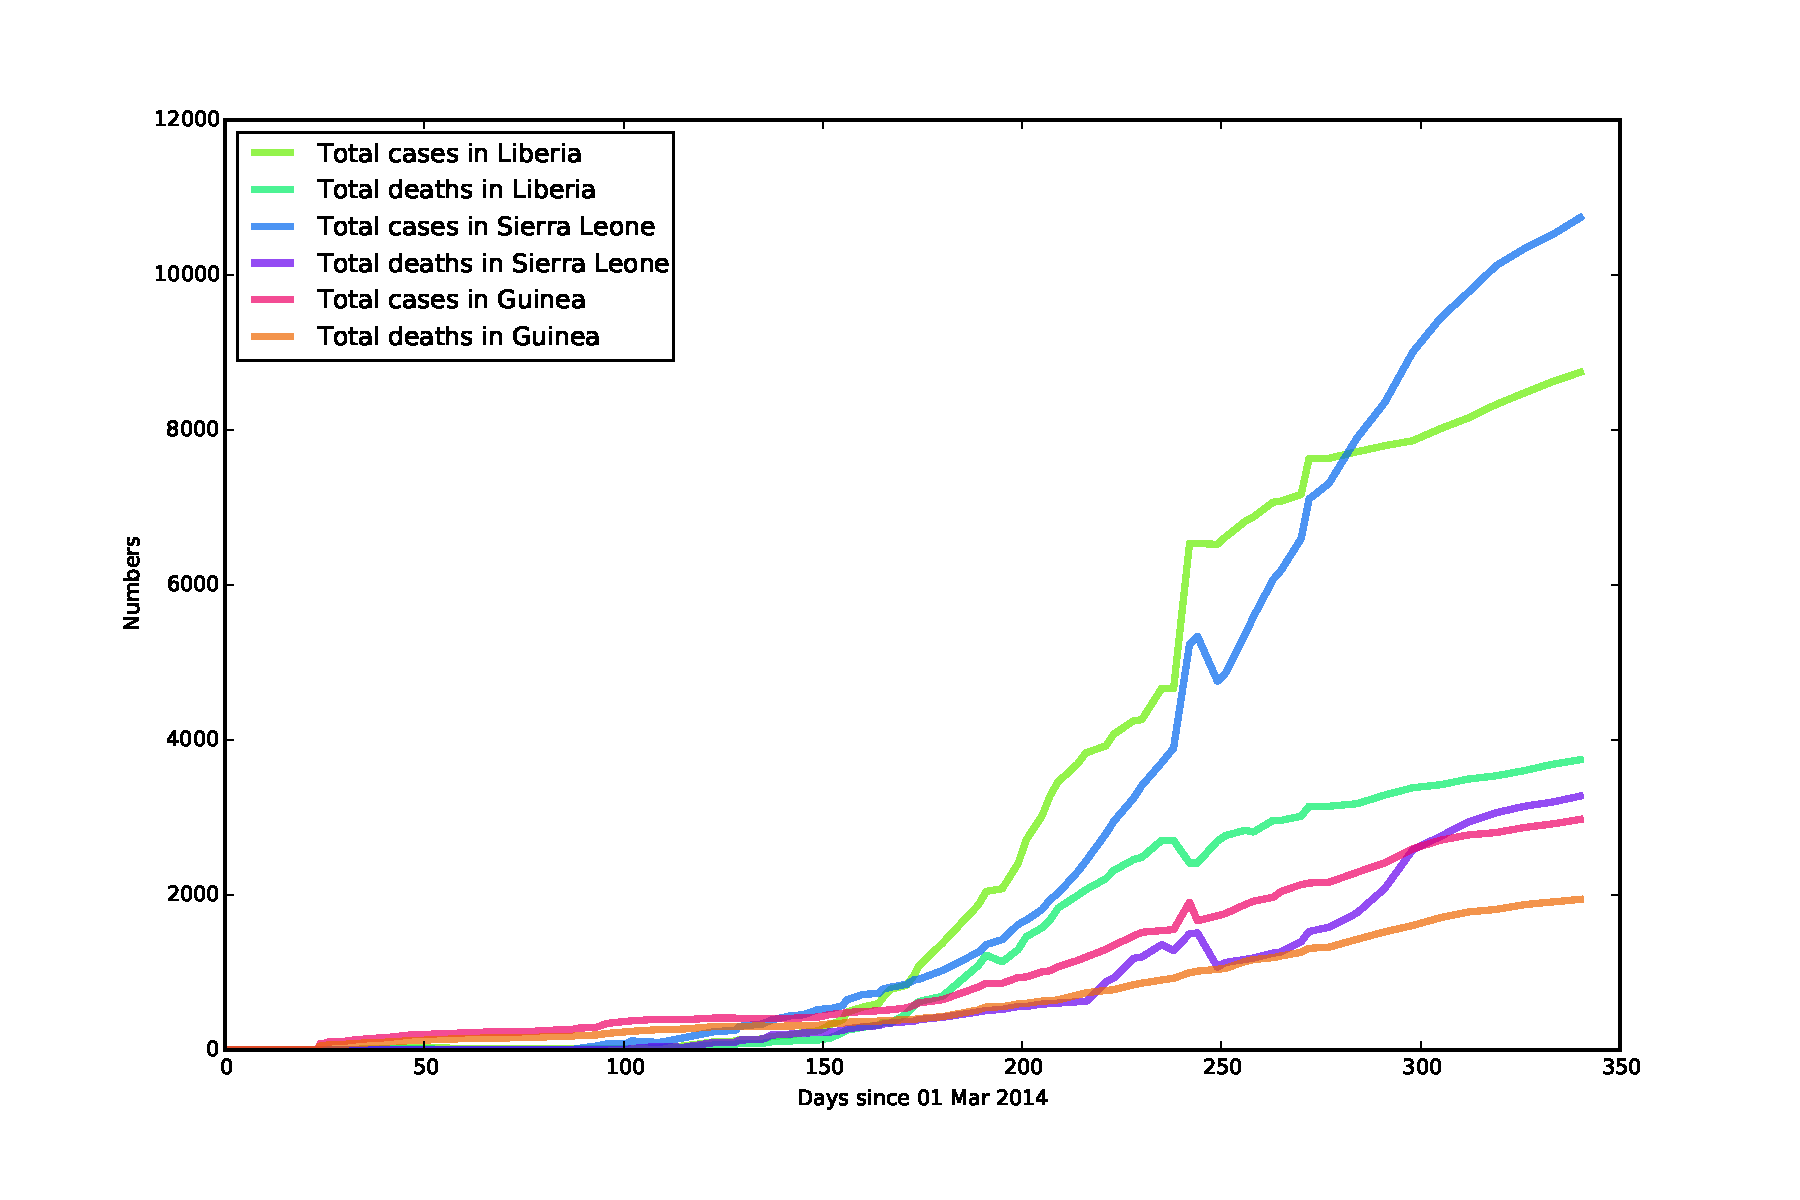
\includegraphics[width=6in]{graph/bstats.pdf}
  \caption{General statistics of Ebola outbreak in 2014}
  \label{stats}
\end{center}  
\end{figure}

Fig.~\ref{stats} shows the basic statistics of the Ebola outbreak in 2014. This is the cumulative cases and deaths in the three countries where the outbreak is the severe.\footnote{The hump of the curve origin from the inconsistency of the data source, it changed on Nov 12 2014.}



\subsection{Transmission}

It is thought that fruit bats of the Pteropodidae family are natural Ebola virus hosts. Ebola is introduced into the human population through close contact with the blood, secretions, organs or other bodily fluids of infected animals such as chimpanzees, gorillas, fruit bats, monkeys, forest antelope and porcupines found ill or dead or in the rainforest.


Ebola then spreads through human-to-human transmission via direct contact (through broken skin or mucous membranes) with the blood, secretions, organs or other bodily fluids of infected people, and with surfaces and materials (e.g. bedding, clothing) contaminated with these fluids.

It is reported that \cite{merler2015spatiotemporal}, 72\%  of infections occurred in households or in the general community , 17.5\% in hospitals, and 10.4\% at funerals. This observation is important for our modelling.

Human-to-human transmission gives rise to the wide spread such disease. It has spread between countries starting in Guinea then spreading across land borders to Sierra Leone and Liberia, by air (1 traveller only) to Nigeria, and by land (1 traveller) to Senegal.\cite{ebolanew}

Figure.~\ref{cities} shows the location of Ebola infected areas. We also got the geological location and other information such as population for the purpose of model calibration.

\begin{figure}[hbt]
\begin{center}
  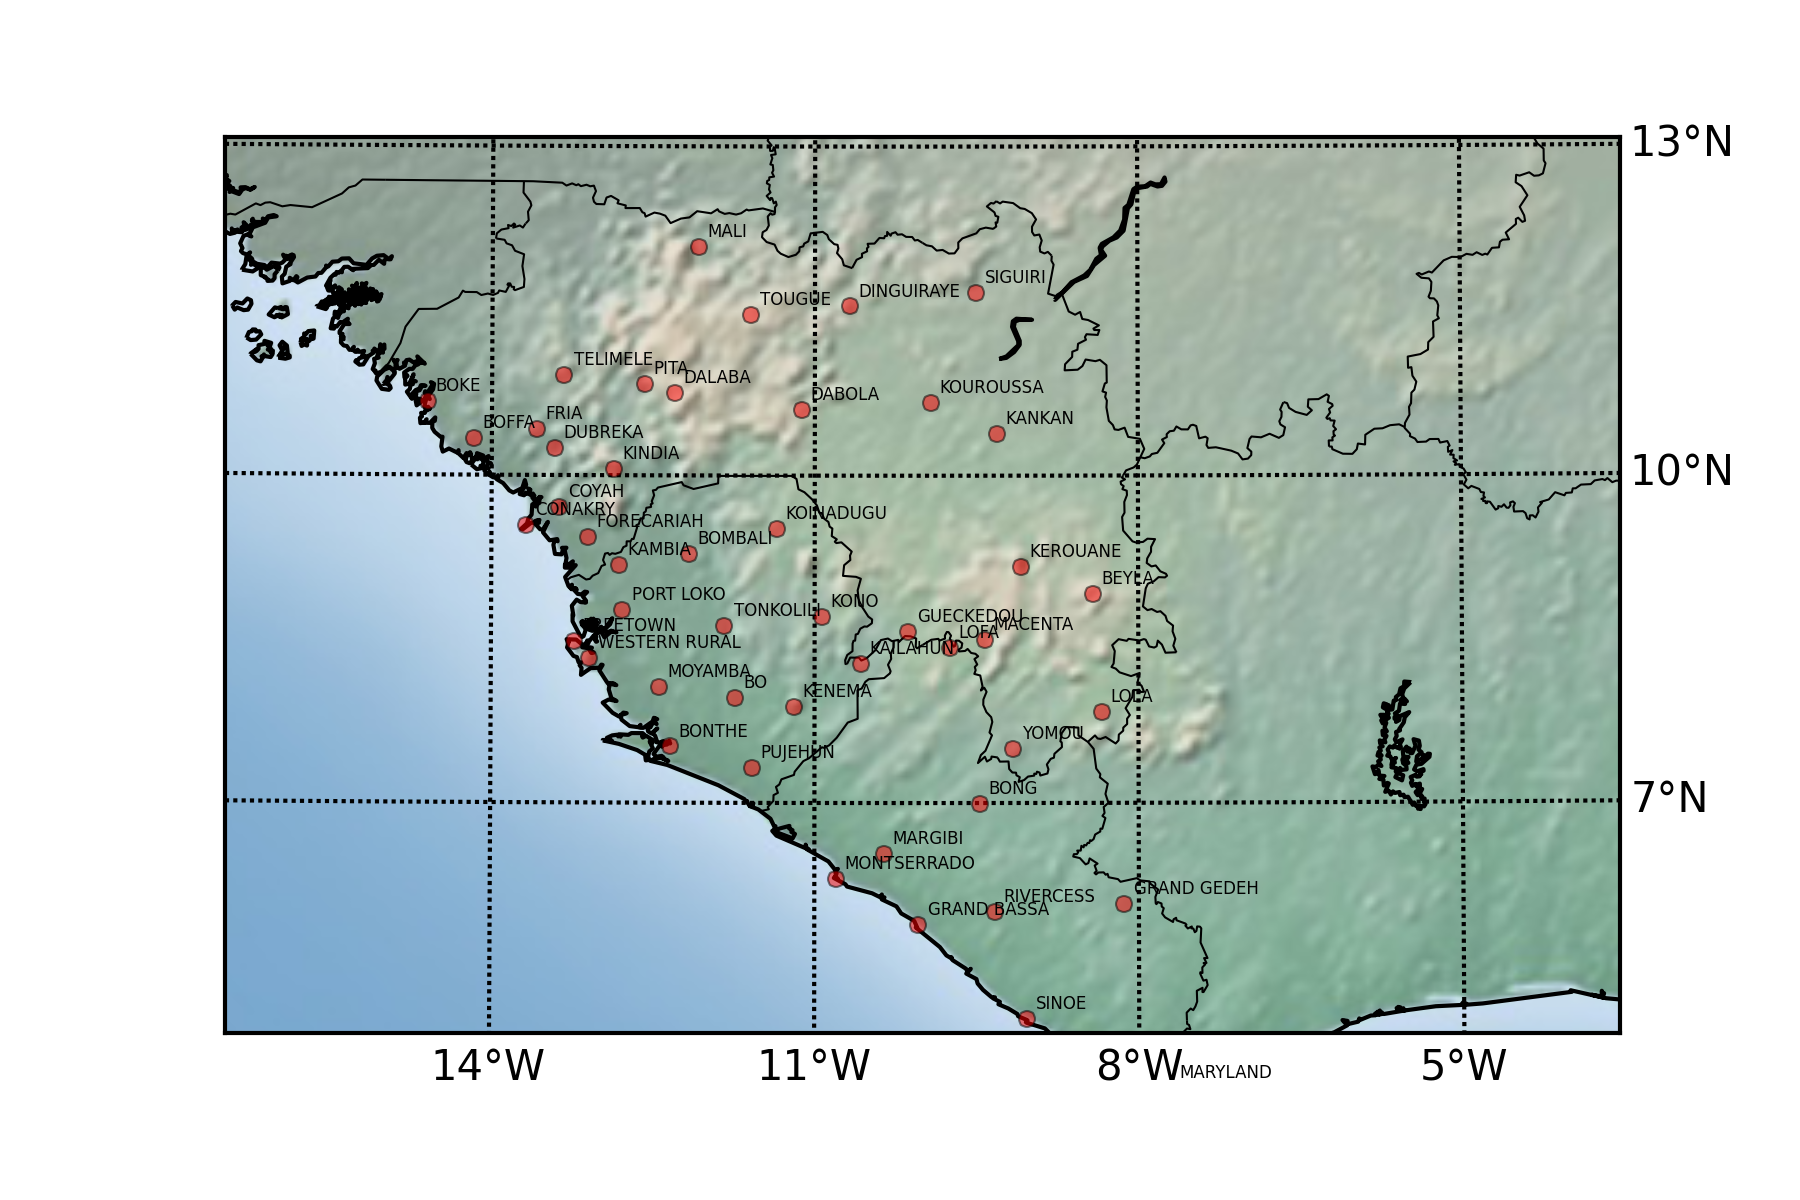
\includegraphics[width=6in]{graph/map3.png}
  \caption{Location of Ebola infected cities}
  \label{cities}
\end{center}  
\end{figure}

From observing the outbreak data in Fig.~\ref{spread} in Appendix , we found there exists a correlation  between infected areas in time. This observation validated that Ebola spread between countries on the land.



\subsection{Medication}

Supportive care-rehydration with oral or intravenous fluids- and treatment of specific symptoms, improves survival. There is as yet no proven treatment available for EVD. However, a range of potential treatments including blood products, immune therapies and drug therapies are currently being evaluated. No licensed vaccines are available yet, but 2 potential vaccines are undergoing human safety testing.

In the modelling, we assume medicine and vaccines are found for treating Ebola.


\section{Problem Formulation}



\subsection{Problem restatement}

The world medical association has announced that their new medication could stop Ebola and cure patients whose disease is not advanced. 

The ultimate goal is to bring Ebola under control. To achieve this goal, a sensible model has to be built, taking not only the spread of the disease, the quantity of the medicine needed, possible feasible delivery systems, locations of delivery, speed of manufacturing of the vaccine or drug into consideration. Then use this model to optimize the eradication of Ebola.

It is natural to break this problem into two parts, the first part focuses on the Ebola itself. For this part, we need to build a model to describe how Ebola spreads and progresses. 

The second part is to build an optimization model to optimize the eradication of Ebola based on the intrinsic properties of Ebola. 
\subsection{Challenges}

Previous research focuses on the statistical level of disease modelling\cite{anderson1992infectious}\cite{lekone2006statistical}\cite{ivorra2014codis}\cite{team2014ebola}\cite{chowell2014transmission}   , thus detailed plan is not easily made from that. So it is challenging to build a fine grind model to assist detailed area-level healthcare plan-making.

The second challenge lies in the spread of disease. Many a time only one traveller from one area to another will cause infection and disease spread in that new area. Traditional statistical models views the population in as a whole, thus they are not able to track this phenomenon. The challenge is to view different areas as a network and consider the effect of population migration\cite{basharpredicting} .


\section{Disease Modelling}
\label{dmodel}
\subsection{Assumptions}

TBD

\subsection{Network Building}

The Ebola infected countries are divided into areas based on its
 political divisions. We denote the areas as nodes, $N_i$. And there exists links between every two nodes. We assign a weight $\sigma_{i,j}$ on each edge to describe the `proximity' of two areas. 
 
Because we mainly consider the population flow, so we adopted the gravity model\cite{anderson2010gravity}\cite{karemera2000gravity} in economics to estimate the population flow between to areas.

$$\sigma_{i,j} = \frac{Po_i^{\beta_1}Po_j^{\beta_2}}{d_{i,j}^{\beta_3}}, i \neq j$$

We denote the population of node $i$ as $Po_i$ and the geological distance between node $i$ and node $j$. For simplification, we set:

$$\beta_1 = 1, \beta_2 = 1, \beta_3 = 2$$

And to calculate the distance between to nodes, we simply used the euclidean distance between two nodes.

We fetched the data of 55 infected areas. The link and the strength of links is visualized in \ref{network}, and the area of circles stands for the population.

\begin{figure}[hbt]
\begin{center}
  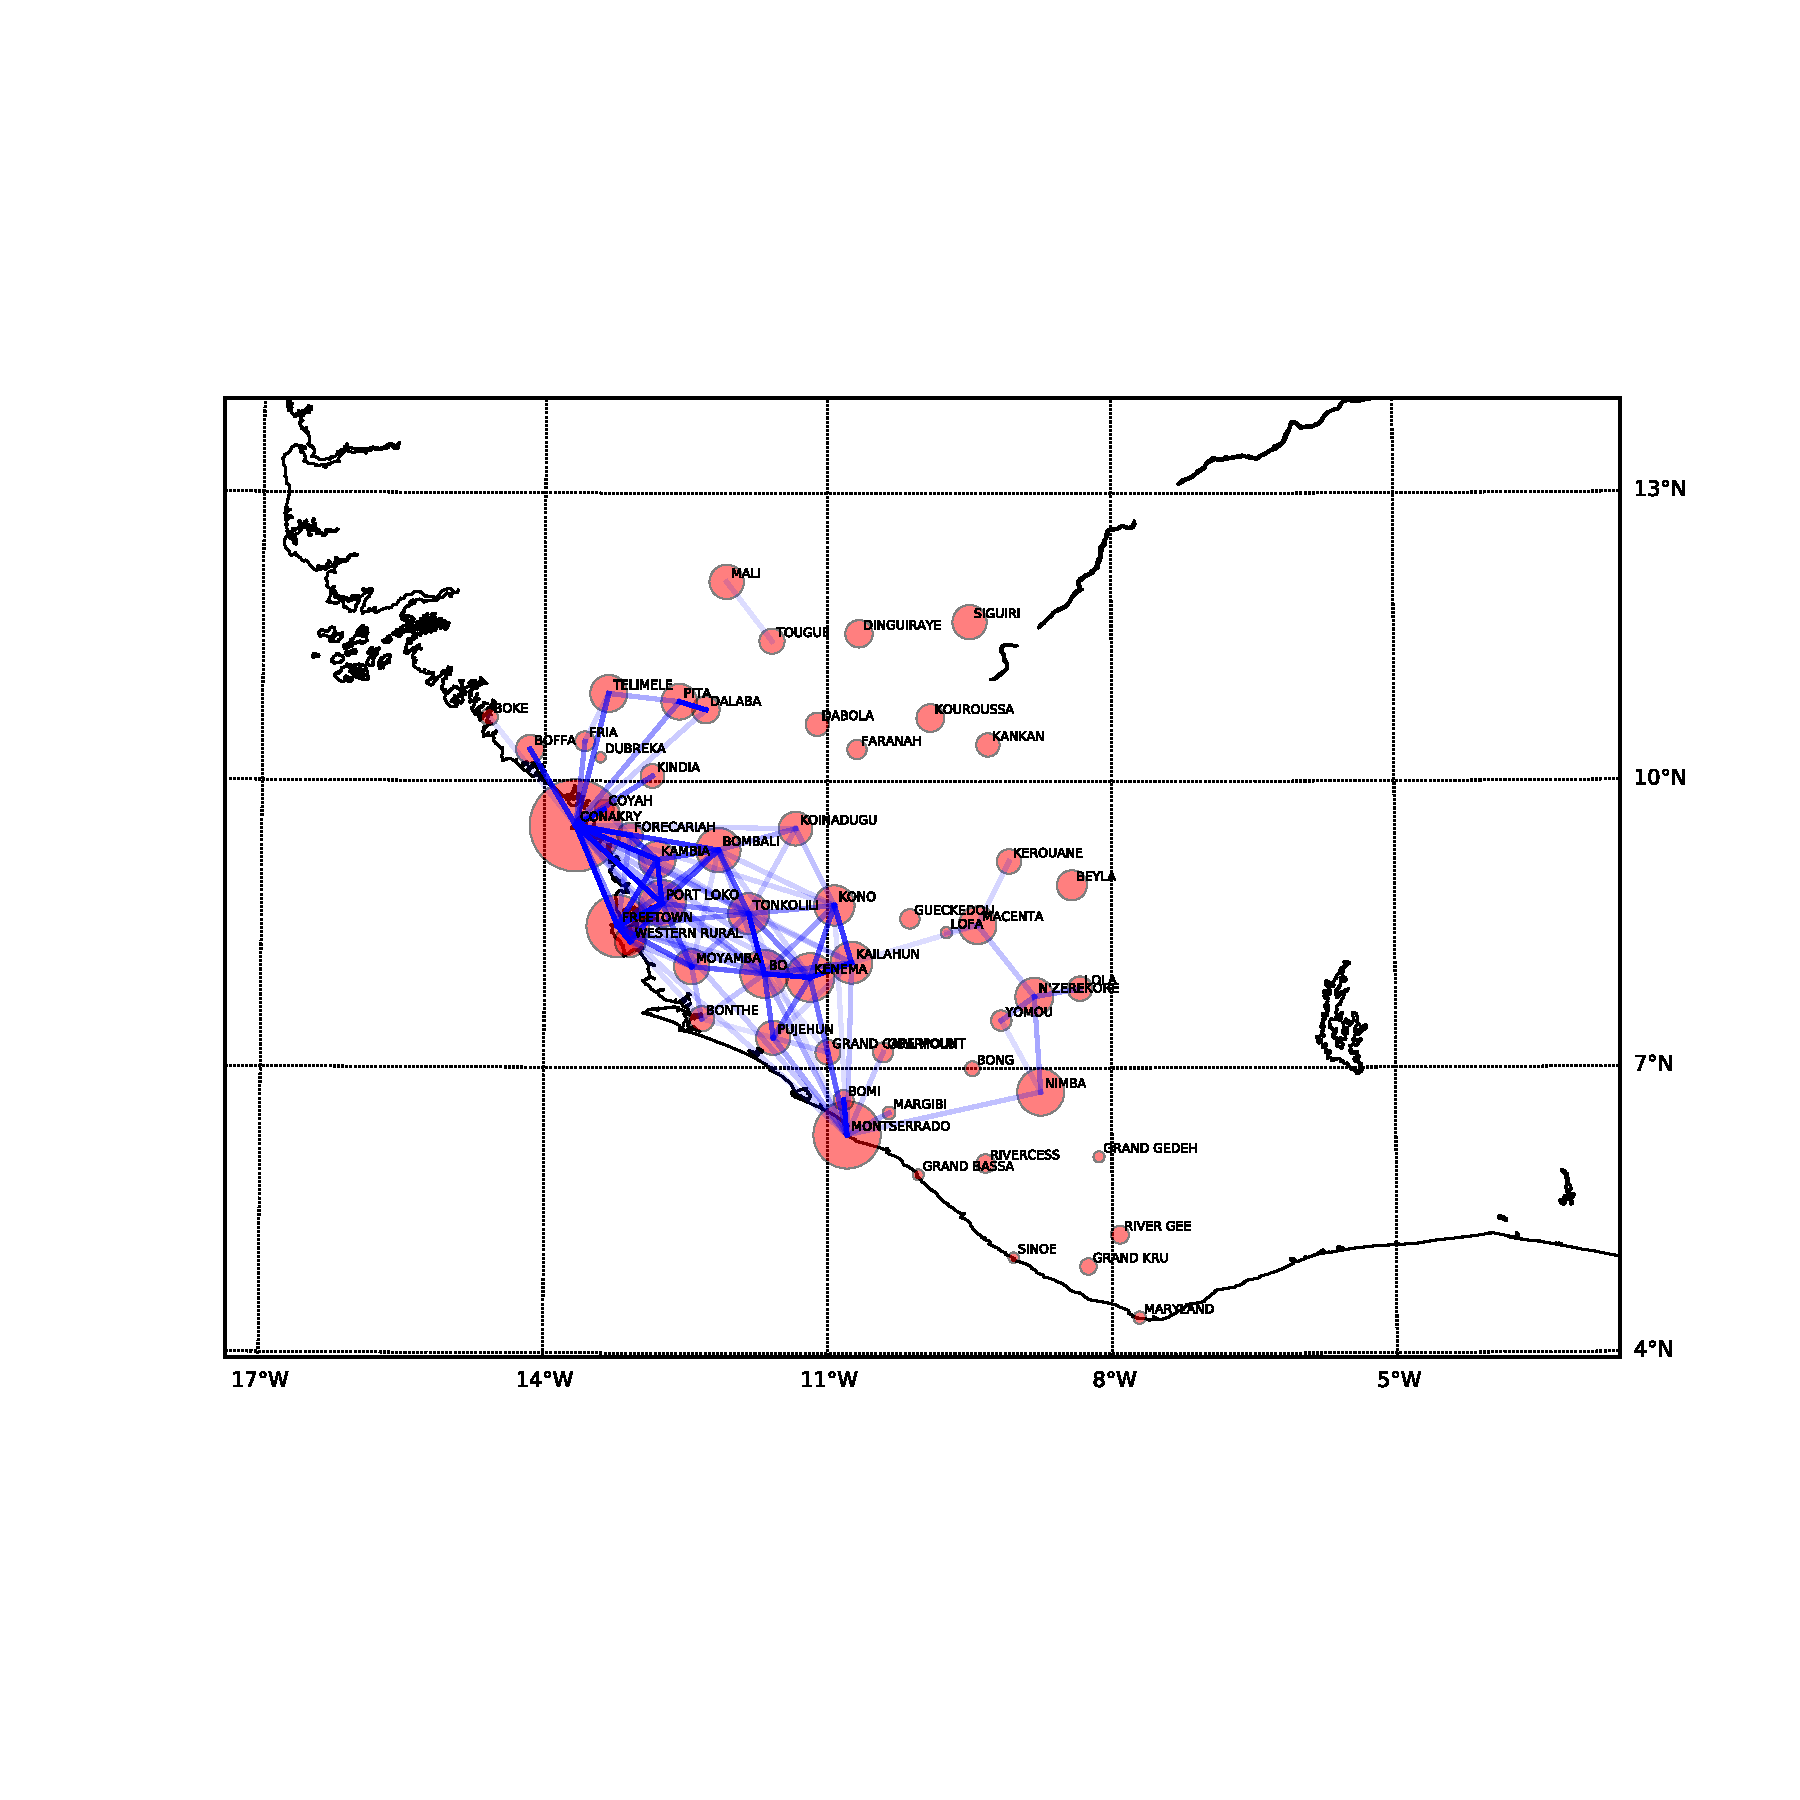
\includegraphics[width=5in]{graph/network2.pdf}
  \caption{Underlying network of population flow}
  \label{network}
\end{center}  
\end{figure}

\subsection{Differential equation model on the network}

We proposed an assisted model based on the network structure and an assisted traditional SIR model.

Other assumptions have to be made. We classify the people into one of the following states:

\begin{itemize}
    \item S: Suspected, not infected but possible for infections
    \item I: Infected, but not go to hospital
    \item H: Infected, and in hospital
    \item R: Removed, recovered or passed away
\end{itemize}

For simplification, we assume the ratio of death or recover is constant and can be observed from statistical data.

\subsubsection{Differential Equation model without considering population flow}

$N$ denotes for the whole population. Because there are three main causes of infection, \emph{household transmission, clinical transmission, and funeral transmission}.

So the rate is proportional to three terms, corresponding to the three causes.

$$\frac{\mathrm{d}S}{\mathrm{d}t} = -\frac{\beta_1 S I}{N}-\frac{\beta_3 S H}{N}  - \frac{\beta_2 S }{N} \frac{\mathrm{d}D}{\mathrm{d}t} $$ 


$$\frac{\mathrm{d}I}{\mathrm{d}t} = \frac{\beta_1 S I}{N} +\frac{\beta_3 S H}{N}  + \frac{\beta_2 S }{N} \frac{\mathrm{d}D}{\mathrm{d}t} - kI$$ 

$$\frac{\mathrm{d}H}{\mathrm{d}t} = kI - \gamma H$$

$$\frac{\mathrm{d}R}{\mathrm{d}t} = \gamma H$$
Because the ratio of death or recover is constant and can be observed from statistical data,so 
$$D =\eta R. $$

\subsubsection{Differential Equation model with considering population flow}

The underlying network is the main dynamic of disease sprawling. 

For every node $V_i \in V$

$$\frac{\mathrm{d}S_i}{\mathrm{d}t} = -\frac{\beta_1 S_i I_i}{N_i}-\frac{\beta_3 S_i H_i}{N_i}  - \frac{\beta_2 S_i }{N_i} \frac{\mathrm{d}D_i}{\mathrm{d}t} + \sum_{j\in V,j\neq i} \theta(\sigma_{i,j} S_j - \sigma_{j,i} S_i) $$ 


$$\frac{\mathrm{d}I_i}{\mathrm{d}t} = \frac{\beta_1 S_i I_i}{N_i} +\frac{\beta_3 S_i H_i}{N_i}  + \frac{\beta_2 S_i }{N_i} \frac{\mathrm{d}D_i}{\mathrm{d}t} - kI_i + \sum_{j\in V,j\neq i} \theta(\sigma_{i,j} I_j - \sigma_{j,i} I_i)$$ 

$$\frac{\mathrm{d}H_i}{\mathrm{d}t} = kI_i - \gamma H_i$$

$$\frac{\mathrm{d}R_i}{\mathrm{d}t} = \gamma H_i$$
Because the ratio of death or recover is constant and can be observed from statistical data,so 
$$D_i =\eta R_i. $$




\subsubsection{Two step model calibration}
The first step of calibration is to determine the parameters for the overall data.

The parameters are $\beta_1,\beta_2,\beta_3, k,\gamma$.

Write the equations in matrix form.
$$\vec{x} =  \begin{pmatrix}
S\\I\\H
 \end{pmatrix}$$ 
 
 $$
 A =  \begin{pmatrix}
0 &-\beta_1 & -\beta_3-\beta_2\eta\gamma \\
0 &\beta_1 -k & \beta_3 + \beta_\eta\gamma \\
0 & k & -\gamma 
 \end{pmatrix}
 $$
 
 Considering the number infected is small comparing to the population. So $$S_i \approx N_i, \frac{\mathrm{d}S_i}{\mathrm{d}t} \approx 0$$
 
 $$\dot{\vec{x}} =  A  \vec{x}$$
 
 The roots of equation $|pI-A| = 0$ are:
 
 $$
 p_1 = 0
 $$
 
 $$
 p_{2,3} = \frac{-k+\beta_1 - \gamma + \sqrt{  (\beta_1 - \gamma - k)^2  - 4(\beta_1 - \gamma - mk + k\gamma) } }{2}
 $$
 
 
 The general solution is 
$$\psi = A\begin{pmatrix}
1\\0\\0
 \end{pmatrix}
 +B\begin{pmatrix}
-m\frac{p_2 + k}{p_2}\\ m \\ p_2 - \beta_1 + k
 \end{pmatrix}
 +C\begin{pmatrix}
-m\frac{p_3 + k}{p_3}\\ m \\ p_3- \beta_1 + k
 \end{pmatrix}
$$


From statistical data we set $\beta_1:\beta_2:\beta_3 = 2:2:1$
 
So $$\psi = B\frac{7}{6}\beta(1+\frac{1}{6.3(\beta - 0.163+\sqrt{\beta^2 + 0.193\beta})}) e^{(\beta - 0.163+\sqrt{\beta^2 + 0.193\beta})t}$$
 
 
We fit the data to the first $2/3$ data and get $$\beta = 0.0612$$ in Fig.~\ref{cfit}.

\begin{figure}[hbt]
\begin{center}
  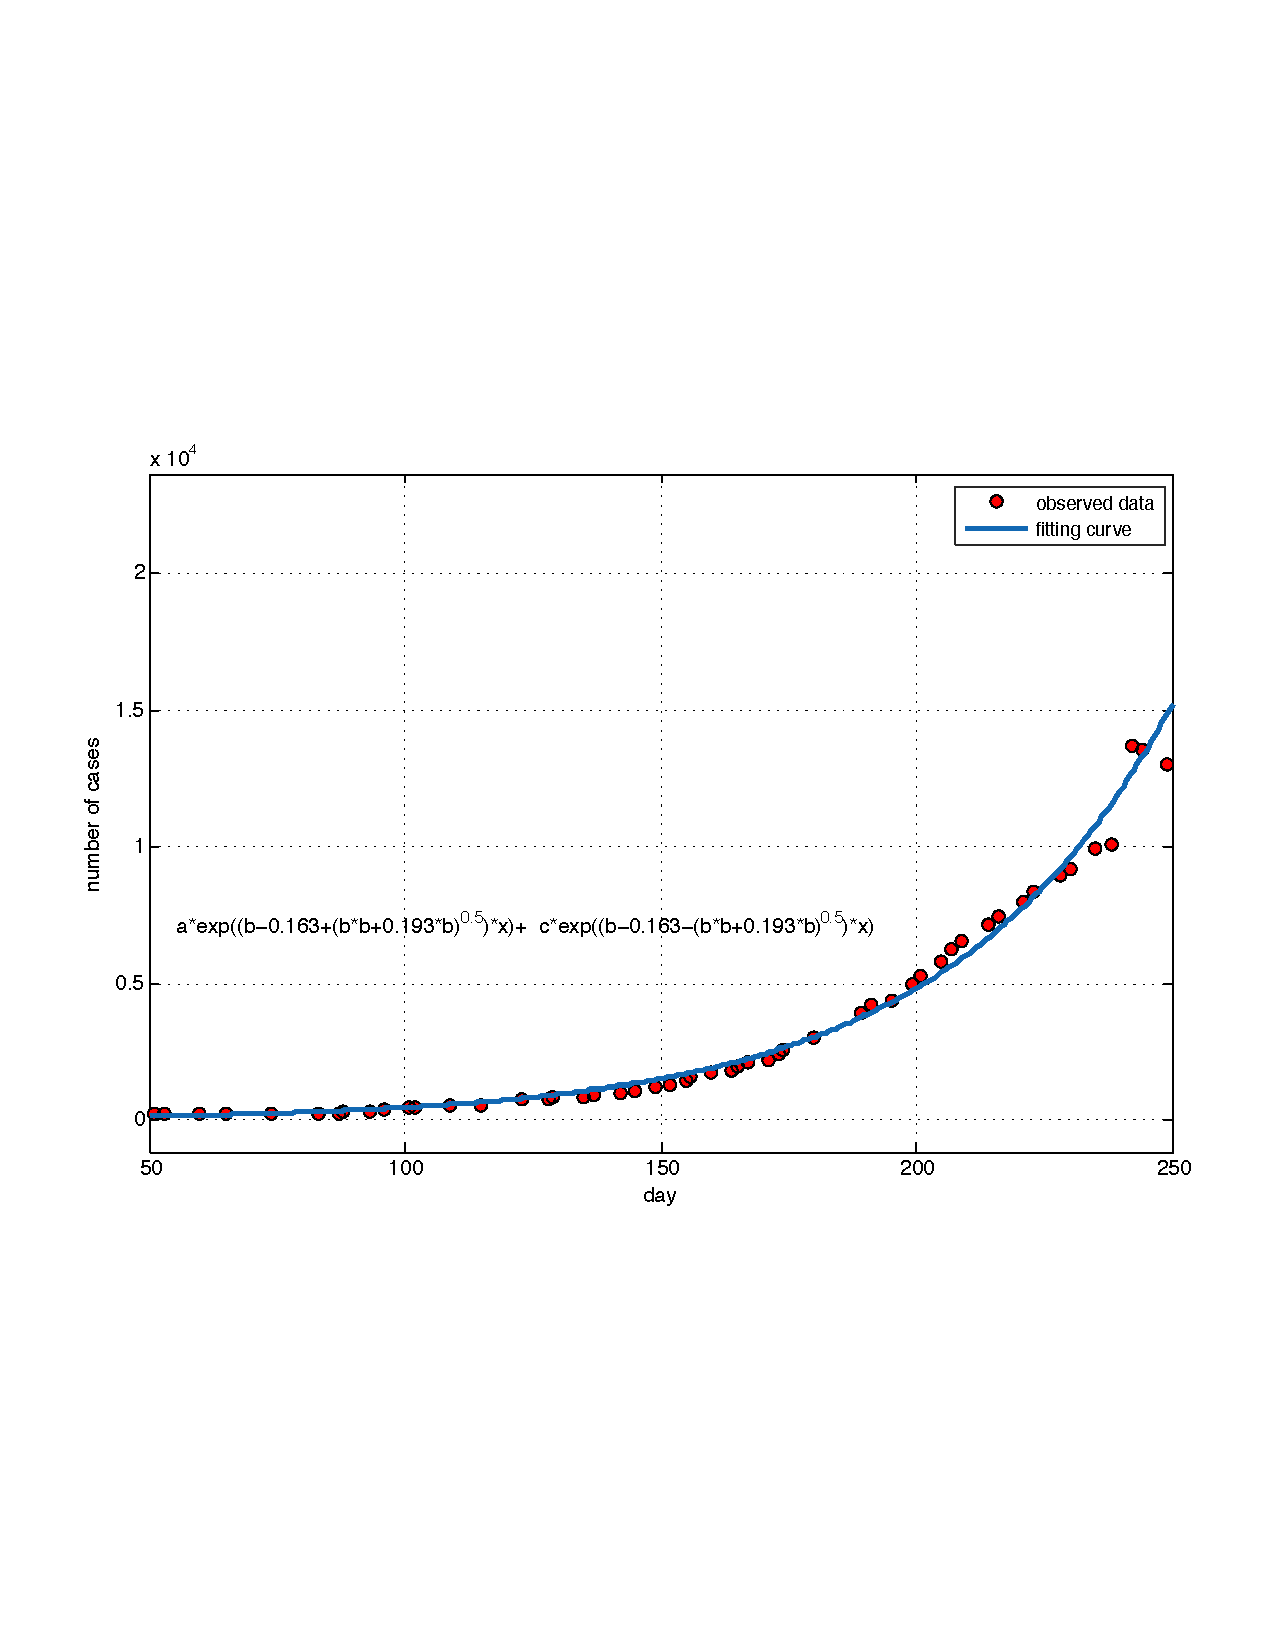
\includegraphics[width=5in]{graph/cfit.pdf}
  \caption{Estimate parameter $\beta$ }
  \label{cfit}
\end{center}  
\end{figure}




The second step of calibration considered the population flow. During the calibration, data of different times at different nodes is used as our initial conditions and after our simulation, we can obtain the prediction for new cases after a fixed time period. And the norm of prediction error can thus be gotten. Thus the best fitted theta can be considered as the one that make the prediction error smallest. The relationship between error and theta can be show as:

We can see that the best theta is about $$\theta = 0.3 \times 10^{-3}$$

Since $\theta$ is such a key parameter which we can conduct the influence ratio between node itself and its neighbourhood, we now give a short discussion. From the right side of second differential equation, we express the influence ratio as

$$
\frac{\sigma_{i,j} I_i}{\beta_1 \frac{S_i I_i}{N_i} } = =  \frac{\theta \sigma_{i,j} N_i}{\beta_1 S_i}
$$

We can estimate the ratio because we konw:

$$
\sigma_{i,j} \sim 10^0, N_i \sim S_i, \beta \sim 10^{-2}, \theta \sim 10^{-3}
$$

Thus the ratio is about $10^{-1}$, meaning that the influence given by a node itself is about $10^1$ times stronger than that obtained from its neighbours.

TBD
(You can mention the concordance in your model later.)


\begin{figure}[hbt]
\begin{center}
  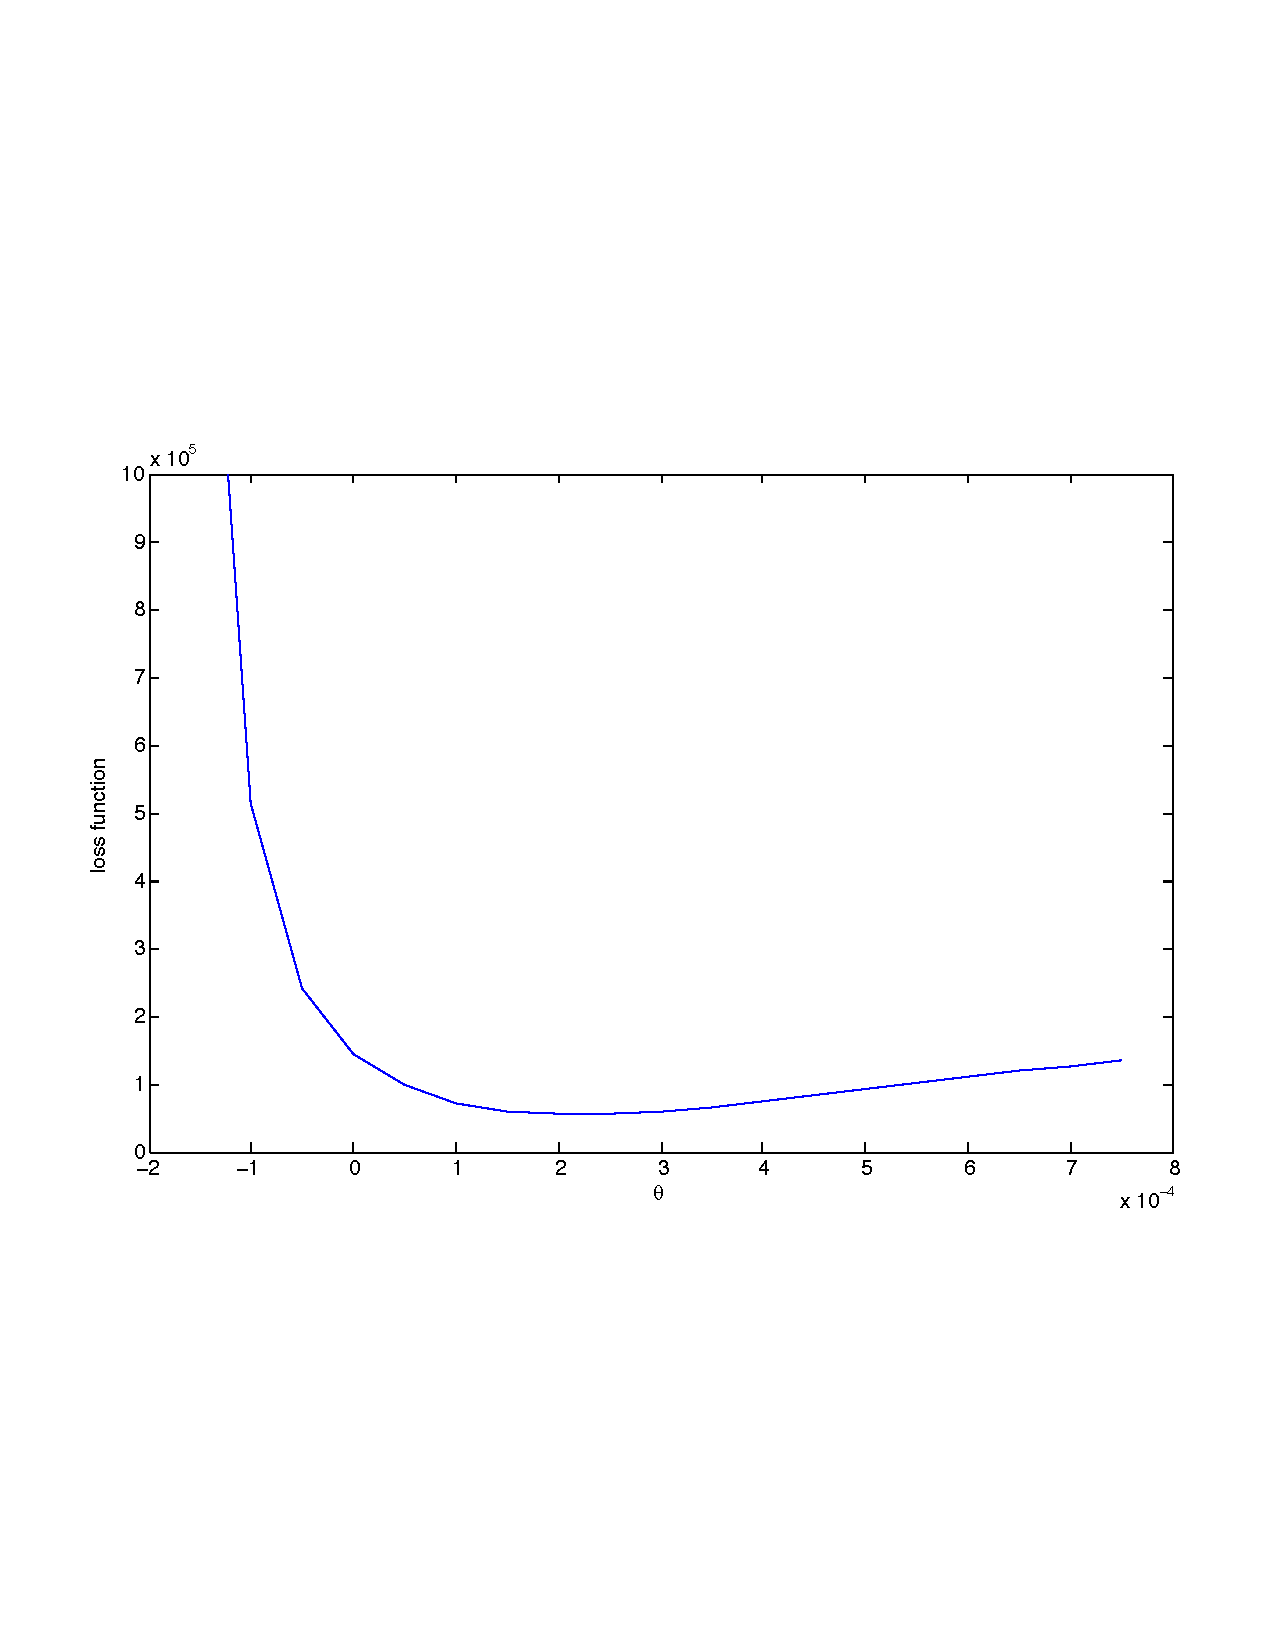
\includegraphics[width=4in]{graph/est3.pdf}
  \caption{Estimated $\theta$}
  \label{est}
\end{center}  
\end{figure}

\label{eth}

\subsubsection{Model Analysis}

During our modeling process using SIHRonNet model, some weakness of these differential model has been exposed clearly, which can be summarized in three aspects:
\begin{itemize}

\item	Bad Timescale:SIHR model does make sense to describe the entire process of a disease outbreak, but its description to the beginning of an outbreak is trivial---- an exponential-like increase can’t give us the detailed information we want.  
\item	No Randomness:In theses models, all the interactions between different states of people is modeled using a proportional relationship, meaning that the model is based on statics. This erases the randomness, which is an unique characteristic at the beginning of an outbreak.
\item	Parameter-based: A lot of parameters are involved in SIHRonNET model making it a hard work to calibrate each of them precisely and even impossible considering the change of parameters with the evolution of time.

\end{itemize}

Above all, though we can still use SIHRonNET model to estimate some trend of the evolution of the illness, a much more timescale-matched, random and parameter-free model is needed to tell us exactly how to eradicate Ebola.
 

\subsection{Cascaded Poisson Process Model}
\subsubsection{Proposed model}
Multi-dimensional Hawkes process\cite{zhou2013learning}\cite{iwata2013discovering} are used to model repeated events and influence between people. It provided inspiration for us to model the infections of disease as a inhomogeneous Poisson Process to track the temporal and spatial behaviour of disease transmissions.

From Fig.~\ref{spread} we can see the new infections, we model the new infections as a diffusion process. We consider the diffusion process using discrete time steps.

One person being infected is a point process, so viewing it from a higher level, the infection is a Poisson Process.

The intensity of the Poisson Process is related to many factors. 

The intensity in one city/area depends on two parts, one part comes from itself, and the second part comes from all other cities. 




$$\mu_{i,t_k} = \lambda_1 \sum_{m = 1}^{ k-1} P_{i,t_m} e^{-\beta(k-m)\Delta t} + \lambda_2 \sum_{j:j\neq i} \sum_{m = 1}^{ k-1} P_{j,t_m} \sigma_{j,i} e^{-\beta(k-m)\Delta t }$$

\subsubsection{Model Calibration}

We do a MLE to fit the data to the model and get $\lambda_1$ and $\lambda_2$.

The likelihood function is:

$$L(\lambda_1, \lambda_2) = \prod_{i \in V} \prod_{k} \frac{(\mu_{i,t_k}\Delta t)^{P_{i,t_k}} e^{-\mu_{i,t_k}\Delta t}}{P_{i,t_k}!}
$$


$$
\log L(\lambda_1, \lambda_2) = \sum_{i \in V} \sum_{k}\left[ {P_{i,t_k} \log{(\mu_{i,t_k}\Delta t)} {-\mu_{i,t_k}\Delta t}} - \log{P_{i,t_k}!} \right]
$$


$$
\frac{\partial \log L(\lambda_1, \lambda_2)}{\partial \lambda_1} = \sum_{i \in V} \sum_{k}\left[ {P_{i,t_k} \frac{ \frac{\partial \mu_{i,t_k}}{\partial \lambda_1}}{\mu_{i,t_k}} {- \frac{\partial \mu_{i,t_k}}{\partial \lambda_1}\Delta t}} \right] 
$$


$$
\frac{\partial \log L(\lambda_1, \lambda_2)}{\partial \lambda_2} = \sum_{i \in V} \sum_{k}\left[ {P_{i,t_k} \frac{ \frac{\partial \mu_{i,t_k}}{\partial \lambda_2}}{\mu_{i,t_k}} {- \frac{\partial \mu_{i,t_k}}{\partial \lambda_2}\Delta t}} \right] 
$$

Solve for equation 1:

$$
\frac{\partial \log L(\lambda_1, \lambda_2)}{\partial \lambda_1} = \sum_{i \in V} \sum_{k}\left[ { \frac{P_{i,t_k}\sum_{m = 1}^{ k-1} P_{i,t_m} e^{-\beta(k-m)\Delta t}}{ \lambda_1 \sum_{m = 1}^{ k-1} P_{i,t_m} e^{-\beta(k-m)\Delta t} + \lambda_2 \sum_{j:j\neq i} \sum_{m = 1}^{ k-1} P_{j,t_m} \sigma_{j,i} e^{-\beta(k-m)\Delta t}}} \right.
$$
$$
\left. {- \left( \sum_{m = 1}^{ k-1} P_{i,t_m} e^{-\beta(k-m)\Delta t} \right)\Delta t} \right] 
$$

solve for equation 2:

$$
\frac{\partial \log L(\lambda_1, \lambda_2)}{\partial \lambda_2} = \sum_{i \in V} \sum_{k}\left[ { \frac{P_{i,t_k}\sum_{j:j\neq i} \sum_{m = 1}^{ k-1} P_{j,t_m} \sigma_{j,i} e^{-\beta(k-m)\Delta t} }{ \lambda_1 \sum_{m = 1}^{ k-1} P_{i,t_m} e^{-\beta(k-m)\Delta t} + \lambda_2 \sum_{j:j\neq i} \sum_{m = 1}^{ k-1} P_{j,t_m} \sigma_{j,i} e^{-\beta(k-m)\Delta t}}} \right.
$$
$$
\left. {- \left( \sum_{j:j\neq i} \sum_{m = 1}^{ k-1} P_{j,t_m} \sigma_{j,i} e^{-\beta(k-m)\Delta t} \right)\Delta t} \right] 
$$

All the terms are positive. So use gradient descent to find the solution.

$$\lambda_1^* = \lambda_1 - \gamma \frac{\partial \log L(\lambda_1, \lambda_2)}{\partial \lambda_1}$$

$$\lambda_2^* = \lambda_2 - \gamma \frac{\partial \log L(\lambda_1, \lambda_2)}{\partial \lambda_2}$$

$\gamma$ is the step size.

We get $\beta$ from statistical data. $$\beta = 0.1$$ 

We set the step size $\gamma = 1\times 10^{-7}$ and started experiments from initial value $\lambda_1 = 0.6$ and $\lambda_2 = 0.01$.

\begin{figure}[hbt]
\begin{center}
  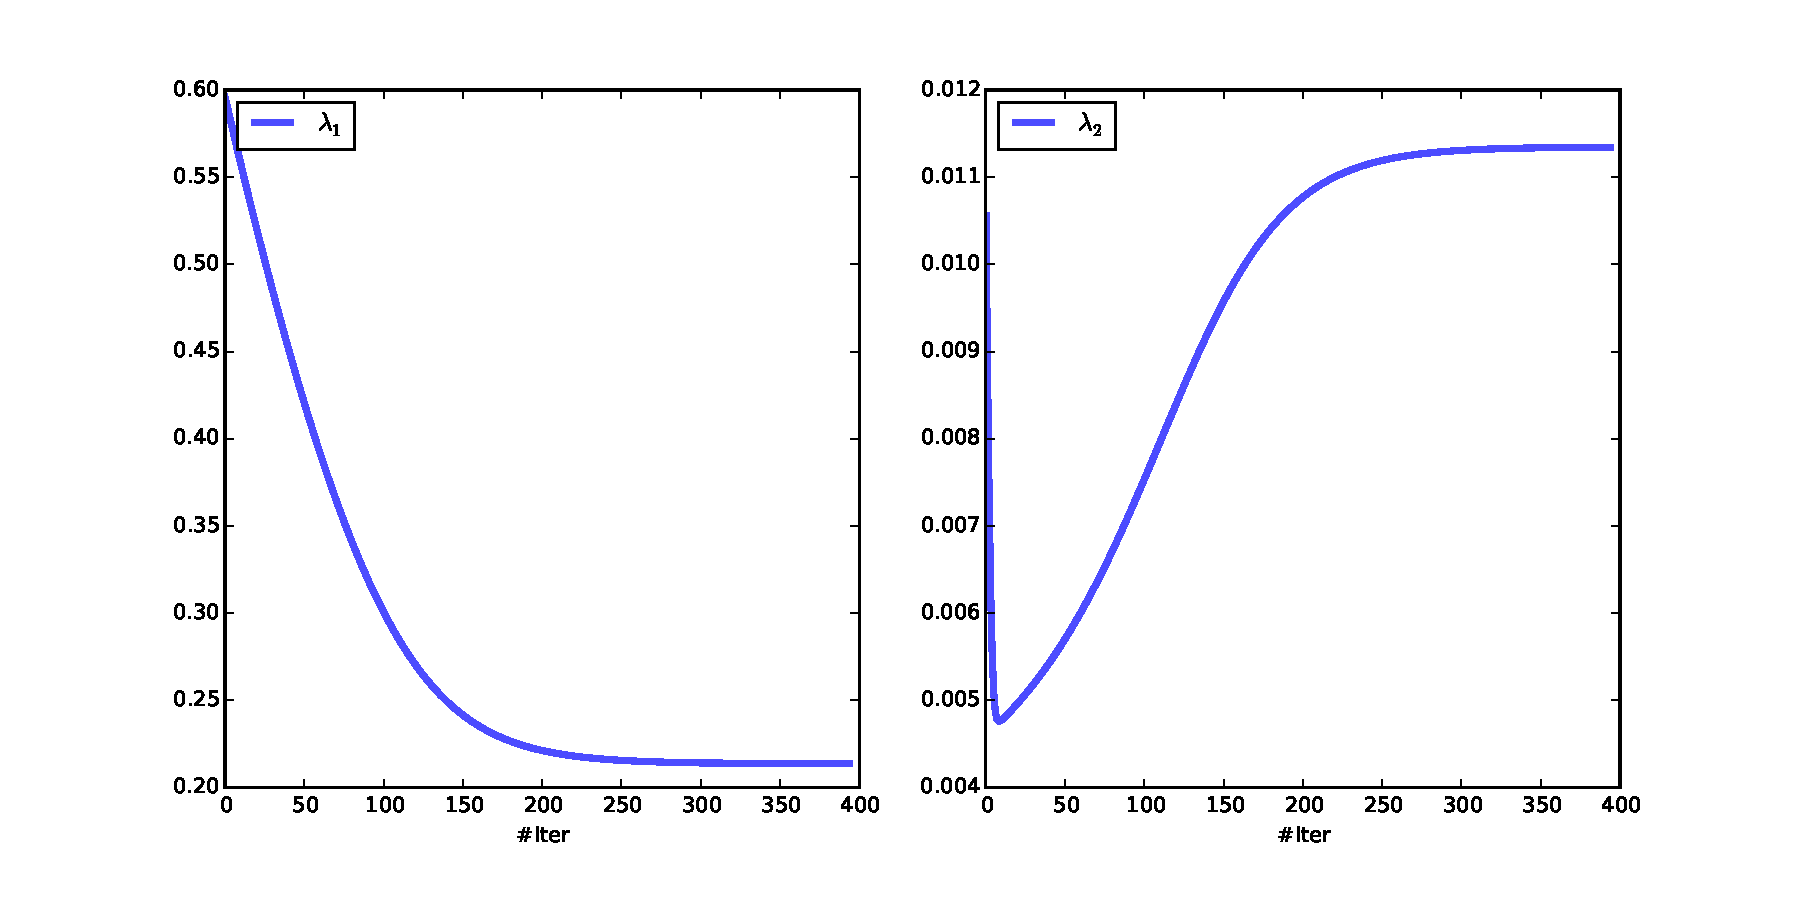
\includegraphics[width=6in]{graph/iter.pdf}
  \caption{Estimated $\lambda_1$ and $\lambda_2$}
  \label{est2}
\end{center}  
\end{figure}

After $400$ iterations, $\lambda_1$ and $\lambda_2$ converge to $0.2136$ and $0.01134$.

$\sigma_{i,j} \sim 10^0$

So $\lambda_1 : \lambda_2 \sigma_{i,j} \sim 10^1$, this is consistent with the result in Section~\ref{eth}.

\subsection{Model Validation}

\subsubsection{Validate the model with observed data}
We use the estimated $\lambda_1$ and $\lambda_2$ to do the estimation of Ebola outbreak for every time step(2 weeks) based on historical data. Fig.~\ref{espread} shows the result of the estimation. The estimated values match well with the ground truth, thus, our model is valid.

\subsubsection{Validate the model with case study}
In the previous section, we showed our model fits very well with the data. Thus, our model is good at tracking the progress of the disease in one area. 

Apart from that, our model has strong predictive abilities because it is built on the network.

We obtained the real data to estimate which areas are prone to be transmitted.

We did a case study on the prediction of our model. 

For example, from observing the data till week 7 since the outbreak, our model produced prediction that there will be outbreak in Freetown and Port Loko. Then in week 8, those two areas are infected indeed. Moreover, the news\cite{ebolanew} confirmed that the outbreak of Ebola in Freetown and Port Loko is due to transmission from adjacent areas.


\begin{figure}[hbt]
\begin{center}
  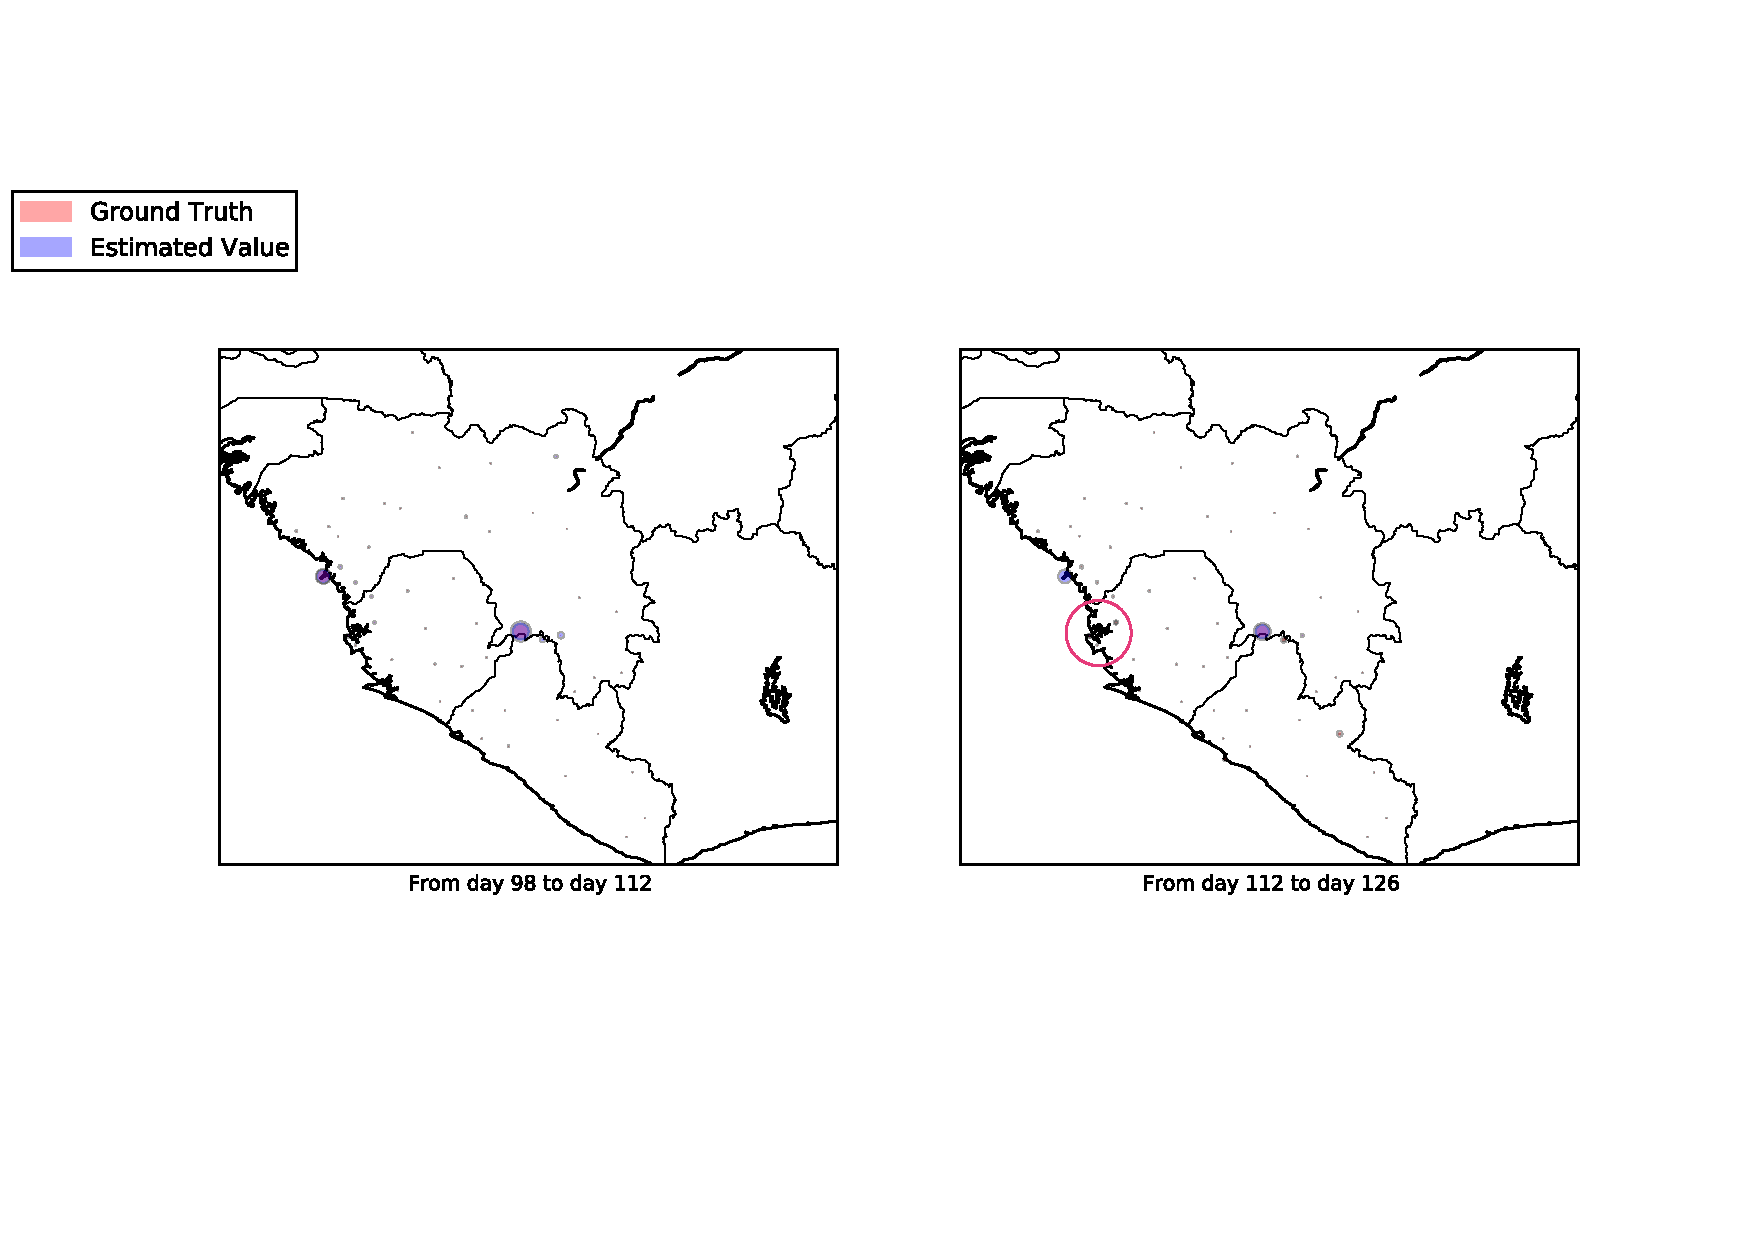
\includegraphics[width=6in]{graph/est22.pdf}
  \caption{Estimated outbreak in Freetown and Port Loko}
  \label{est22}
\end{center}  
\end{figure}


\subsubsection{Validate by comparing two models}


\subsection{Model Analysis}

\subsubsection{Sensitivity analysis}

To 





\begin{figure}[hbt]
\begin{center}
  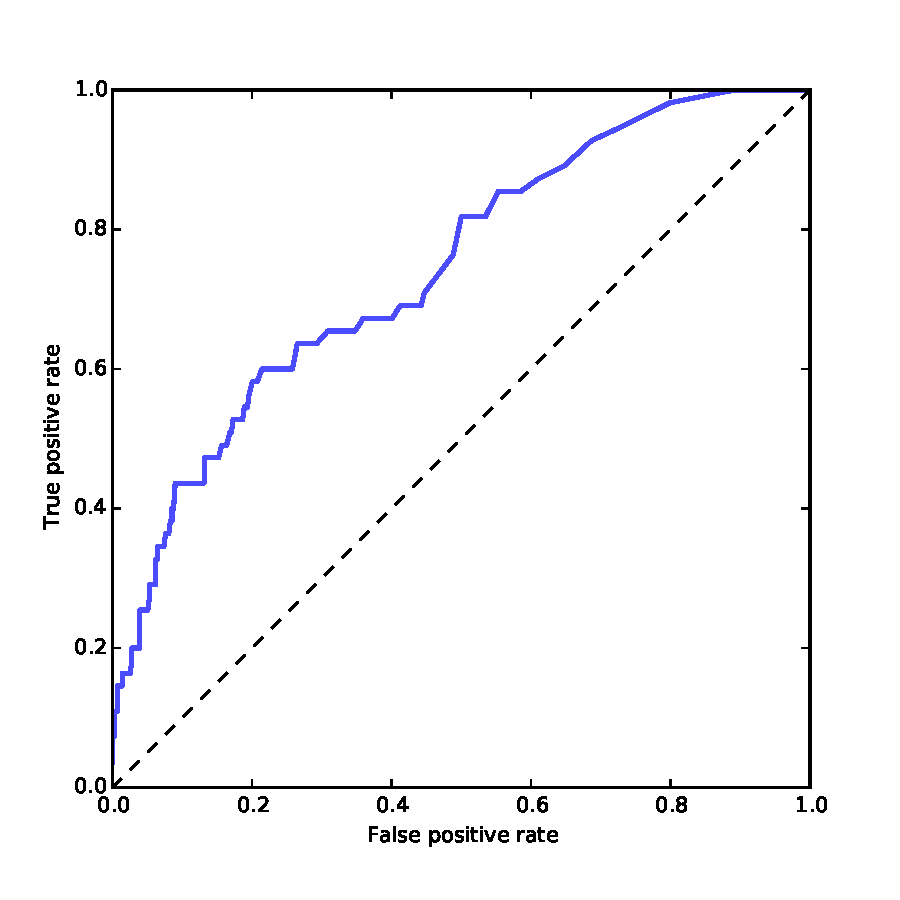
\includegraphics[width=4in]{graph/roc.pdf}
  \caption{ROC of prediction}
  \label{roc}
\end{center}  
\end{figure}

\begin{figure}[hbt]
\begin{center}
  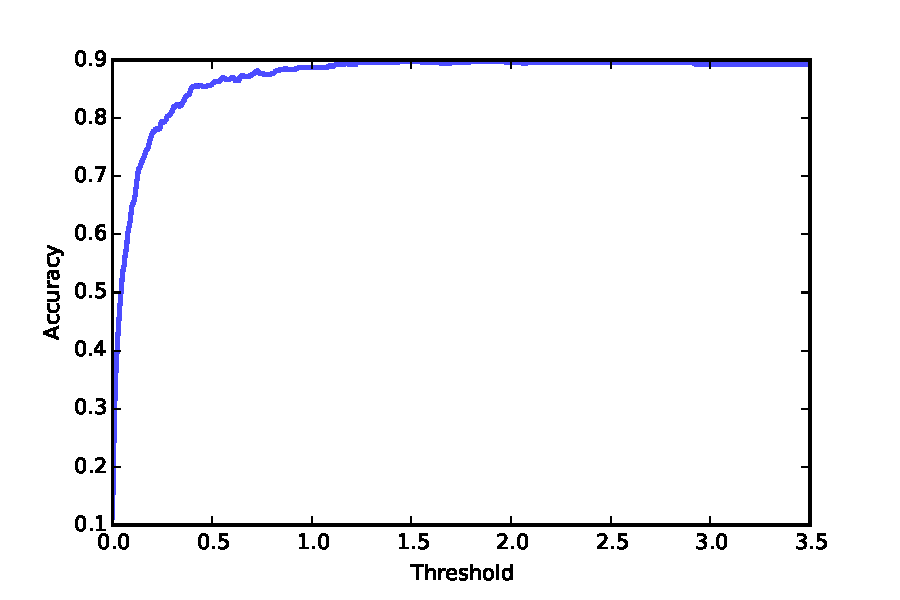
\includegraphics[width=4in]{graph/acc.pdf}
  \caption{Accuracy of prediction}
  \label{acc}
\end{center}  
\end{figure}


\begin{figure}[hbt]
\begin{center}
  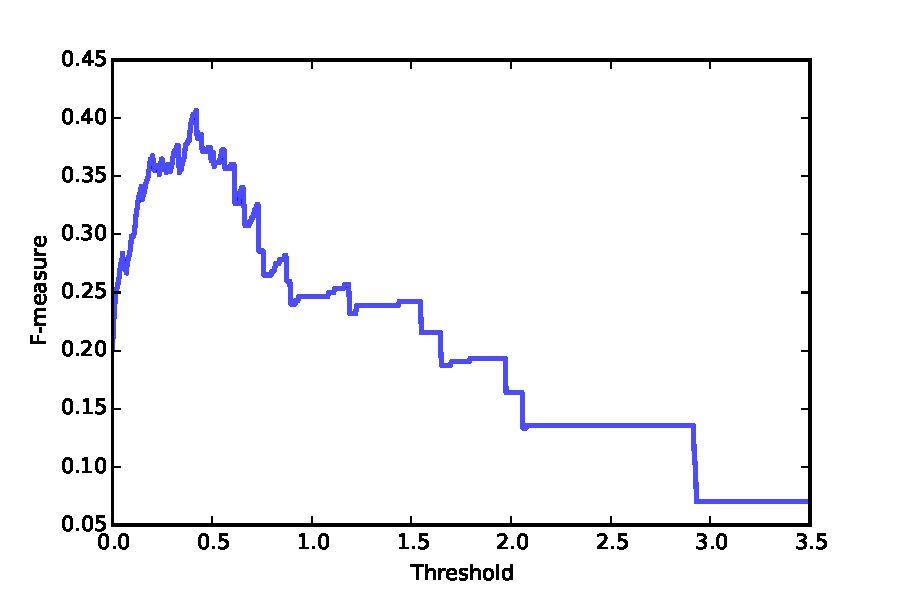
\includegraphics[width=4in]{graph/fmeasure.pdf}
  \caption{F-measure of prediction}
  \label{fm}
\end{center}  
\end{figure}


\begin{figure}%[hbt]
\begin{center}
  
\includegraphics[width=1in]{graph/elabel.pdf}

  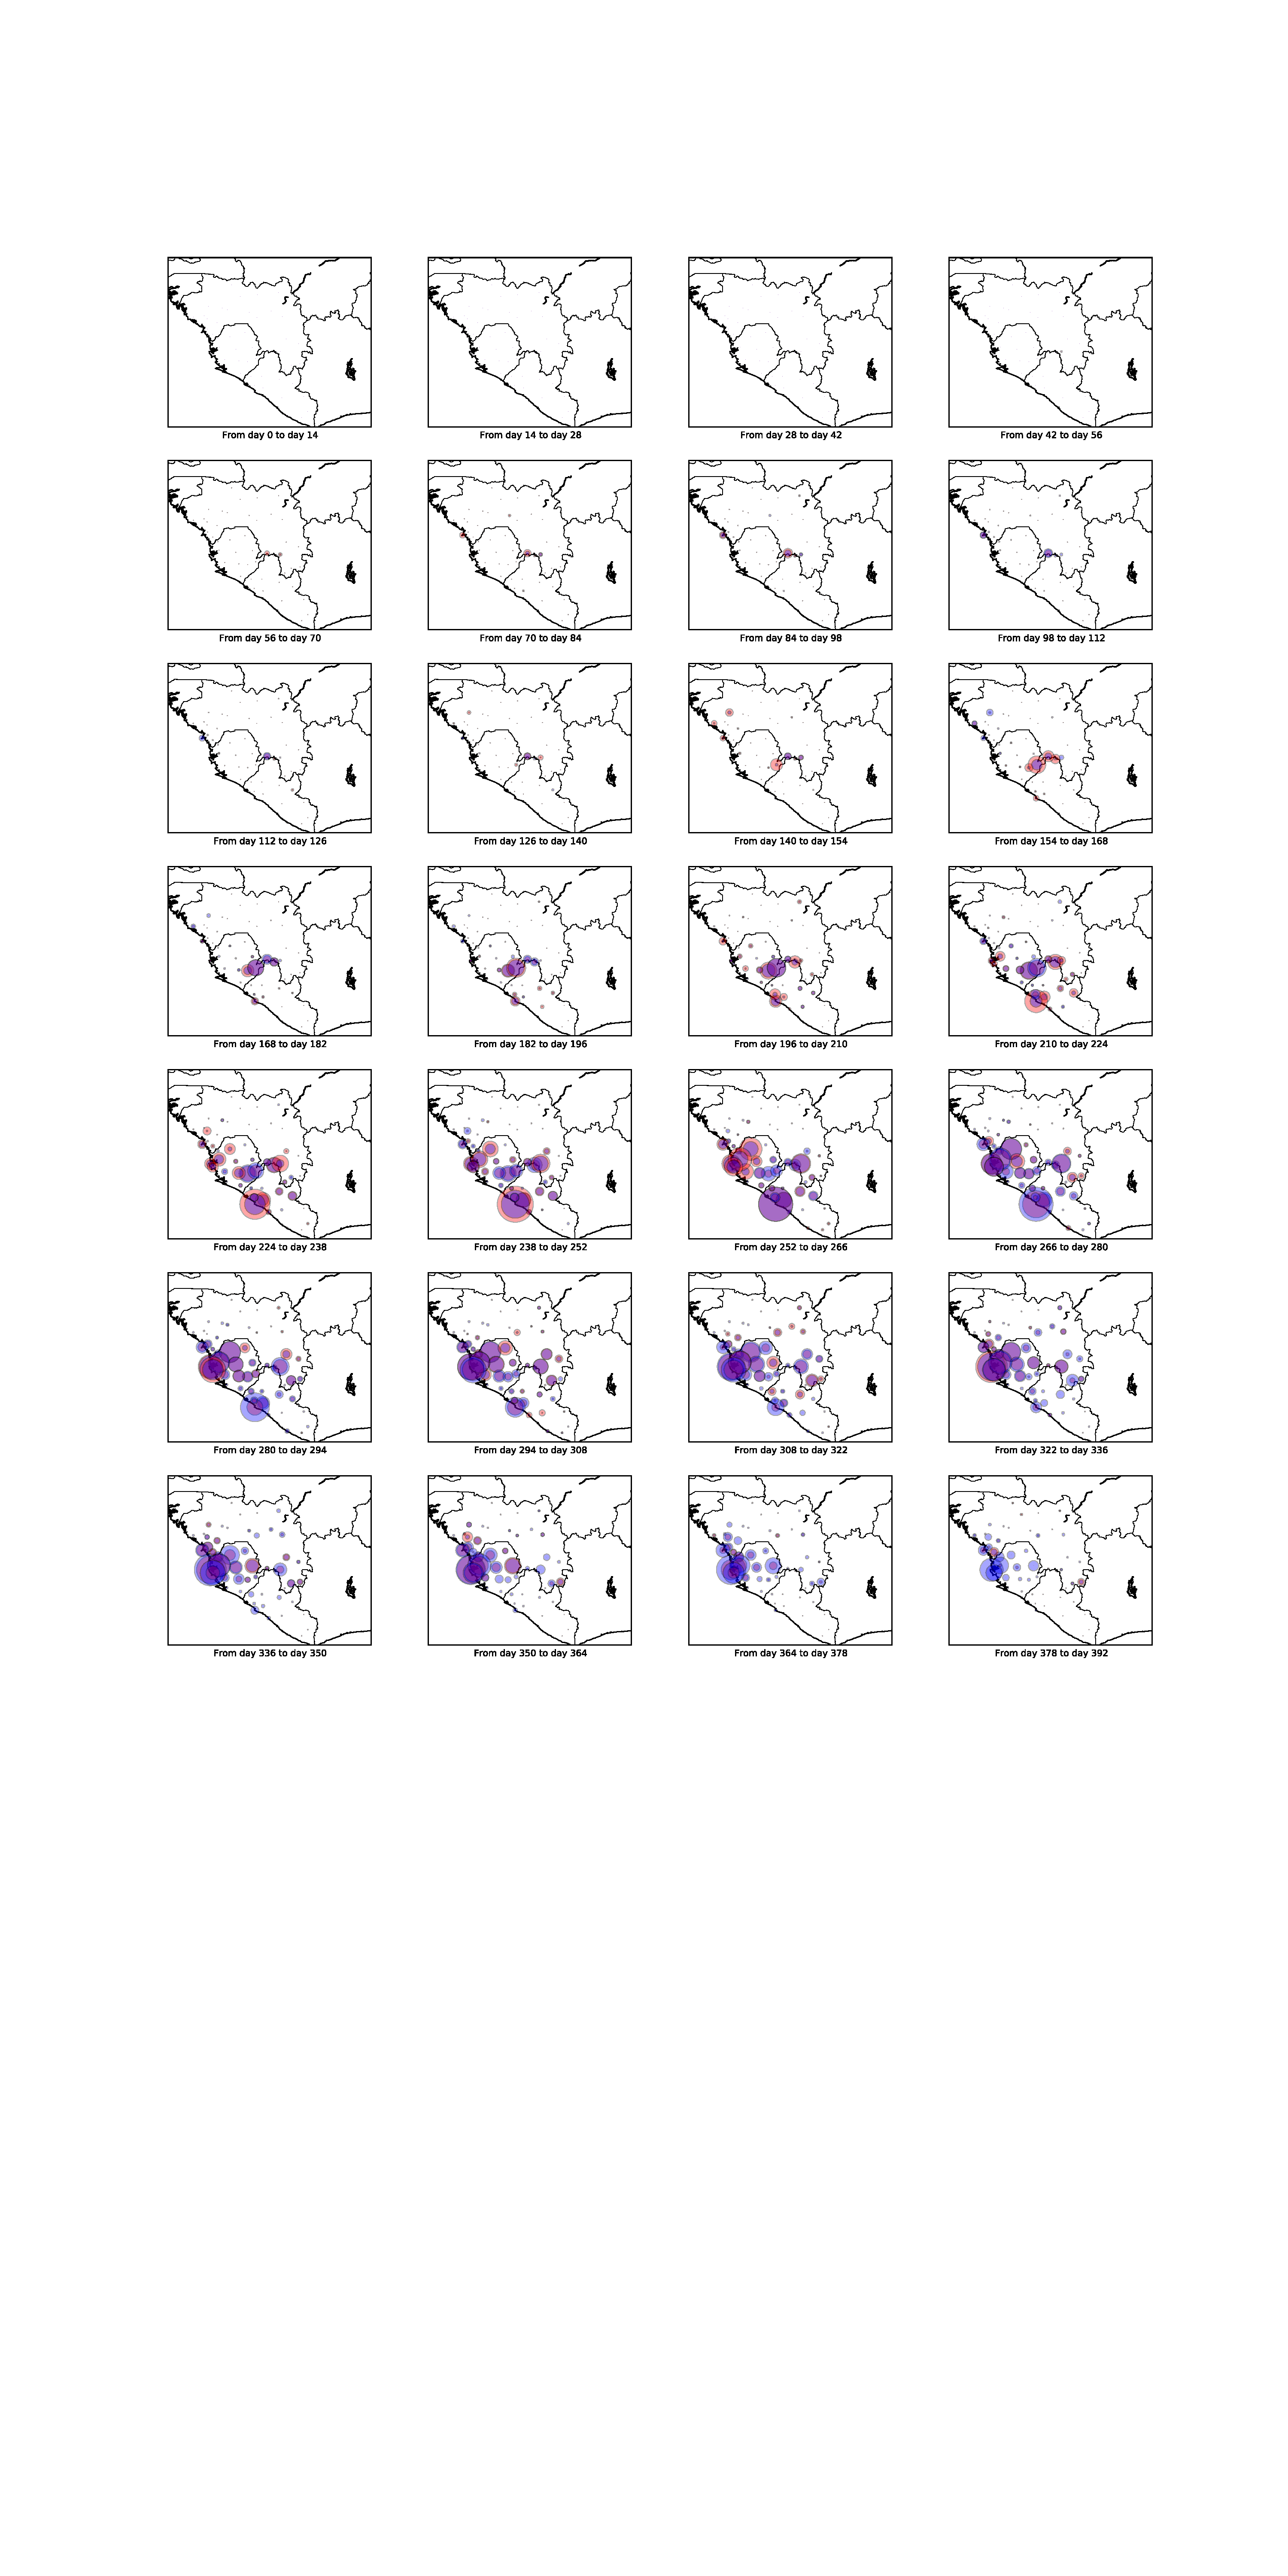
\includegraphics[width=5.9 in]{graph/ee.pdf}
  \caption{Estimated spatiotemporal spread of Ebola. The red marker means the ground truth and the blue marker means the estimated value. And the area of the circle means the scale of the outbreak. For the well estimated outbreaks, the two colors mix to make purple.}
  \label{espread}
\end{center}  
\end{figure}


\section{Disease Controlling}

\subsection{Objective}
We break the control of the disease into two steps with considering different factors. 

The first step is two temporarily bring the ebola under control. We formalize this problem as following:

\emph{Problem~1}

Given the Ebola spread models in Section~\ref{dmodel}, and a certain medication model $M$, with the current situation $P_{j,t_m}, j \in V, t_m \leq T$. Propose the best allocation of medicine, to minimize the loss $L(T')$ at time $T'$, $T' > T'$, and determine the impact of important factors to the disease controlling process.


\emph{Problem~2}

The second step is to ultimately eliminate the Ebola disease from the earth. This goal is formalized as following:

Given the Ebola spread models in Section~\ref{dmodel}, and a certain medication model $M$, with the current situation $P_{j,t_m}, j \in V, t_m \leq T$. Propose the best allocation of medicine, to minimize the cumulative loss $\int_{T}^{\infty} L(t) dt $, and determine the critical factors having effect on whether   the disease can be eliminated, i.e, $\text{lim}_{t\rightarrow \infty} L(t) = 0 $

For different perspectives in Problem $1$ and $2$, either proposed disease spreading model has advantages, so we will use the most suitable model for  analysing different tasks in those problems.


\subsection{Disease Controlling based on Cascaded Poisson Process Model}

\label{str}
The mechanism of medicine on a patient $P$ : If the disease is not advanced (less than $T_0$), $P$ is recovered and removed from the system. And $P$ will not have any effects on the next time step.

We set $T_0$ to two weeks. 

If the observation window is long, for example if $\Delta t= T_0$, then only patients in last time step can be cured.

Assume we have $m$ amount of medicines for $m$ patients. And we want to maximize the effect of these medicines.

$$\mu_{i,t_k} = \lambda_1 \sum_{m = 1}^{ k-1} P_{i,t_m} e^{-\beta(k-m)\Delta t} + \lambda_2 \sum_{j:j\neq i} \sum_{m = 1}^{ k-1} P_{j,t_m} \sigma_{j,i} e^{-\beta(k-m)\Delta t}$$

Denote $C_{i,t_m}$ is the number of patients cured in area $i$ and time step $m$, $C_{i,t_m} \leq P_{i,t_m}$.

$$\sum_i C_{i,t_m} = C_{t_m}$$

$$\mu'_{i,t_k} = \lambda_1 \sum_{m = 1}^{ k-1} (P_{i,t_m} - C_{i,t_m}) e^{-\beta(k-m)\Delta t} + \lambda_2 \sum_{j:j\neq i} \sum_{m = 1}^{ k-1} (P_{j,t_m}-C_{i,t_m}) \sigma_{j,i} e^{-\beta(k-m)\Delta t}$$

$$
E[\sum_n {P'_{n,t_k}}] = \sum_i \mu'_{i,t_k} = \lambda_1 \sum_n \sum_{m = 1}^{ k-1} P'_{i,t_m} e^{-\beta(k-m)\Delta t} + \lambda_2 \sum_n \sum_{j:j\neq i} \sum_{m = 1}^{ k-1} P'_{j,t_m} \sigma_{j,i} e^{-\beta(k-m)\Delta t}
$$
$$
\lambda_1 \sum_n \sum_{m = 1}^{ k-1} (P_{i,t_m} - C_{i,t_m}) e^{-\beta(k-m)\Delta t} + \lambda_2 \sum_n \sum_{j:j\neq i} \sum_{m = 1}^{ k-1} (P_{j,t_m} - C_{i,t_m}) \sigma_{j,i} e^{-\beta(k-m)\Delta t}
$$

The coefficient of $C_{i,t_m}$ is $\lambda_1 e^{-\beta(k-m)\Delta t} + \lambda_2 \sum_{j:j\neq i} e^{-\beta(k-m) \Delta t}$

Strategy: 

find the node with the max weight:
 $$w_{c,i} = \lambda_1 + \lambda_2 \sum_{j:j\neq i} \sigma_{j,i}$$
 
In this case, the weight of areas is only related to $\sum_{j:j\neq i} \sigma_{j,i}$.


If the observation window is smaller, for example $\Delta t = \frac{1}{u} T_0$, then patients in last $u$ time steps can be cured. 

$$w_{c,i,m} = \lambda_1 e^{-\beta(k-m)\Delta t} + \lambda_2 \sum_{j:j\neq i} e^{-\beta(k-m) \Delta t}, k-u\leq m < k$$


TBD


Vaccination:

The vaccination is applied to a number of citizens in a certain area $i$ at a certain time $t_m$, then they are immune to Ebola in the future $t,t>t_m$. 

$$Va_{i,t_m} = \delta Po_i $$
$$\sum_i Va_{i,t_m} = Va_{t_m} $$
 

Then 
$$\mu'_{i,t_k} =(1 - \delta) \mu_{i,t_k} , k > m $$ 


$$
E[\sum_{i \in n} {P'_{n,t_k}}] = \sum_{i \in n} \mu'_{i,t_k} = \lambda_1 \sum_{i \in n} \left( 1 - \frac{Va_{i,t_{ < k}}}{Po_i} \right) \sum_{m = 1}^{ k-1} P_{i,t_m} e^{-\beta(k-m)\Delta t} $$
$$ + \lambda_2 \sum_{i \in n}\left( 1 - \frac{Va_{i,t_{< k}}}{Po_i}\right) \sum_{j:j\neq i} \sum_{m = 1}^{ k-1} P_{j,t_m} \sigma_{j,i} e^{-\beta(k-m)\Delta t}
$$

The benefit from $Va_{i,t_{ < k}}$ is:

$$
w_{v,i} = \lambda_1 \sum_{m = 1}^{ k-1} \frac{P_{i,t_m}}{Po_{i}} e^{-\beta(k-m)\Delta t} + \lambda_2 \sum_{j:j\neq i} \sum_{m = 1}^{ k-1} \frac{P_{j,t_m}}{Po_{i}} \sigma_{j,i} e^{-\beta(k-m)\Delta t} = \frac{E[P_{i,t_k}]}{Po_{i}}
$$





\subsubsection{Experimental validation}

We adopted the strategy in Section \ref{str} to test their effects on disease controlling.

We tested the proposed method against other trivial methods such as assign medicine proportional to number of new cases and showed our method is optimal.

If the number of medicine is fixed, it can be inferred from Figure.\ref{med} that no matter how much the amount of the drug is, our strategy is always the best.

In Figure.~\ref{ev}, we tested the proposed vaccination method against other general methods such as assign vaccine proportional to number of new cases and showed our method is optimal.

We can draw a conclusion from Figure.~\ref{med2} that when the amount of vaccine is a constant number.On the scale of the amount, our proposed vaccination method is better than other methods.



\begin{figure}[hbt]
\begin{center}
  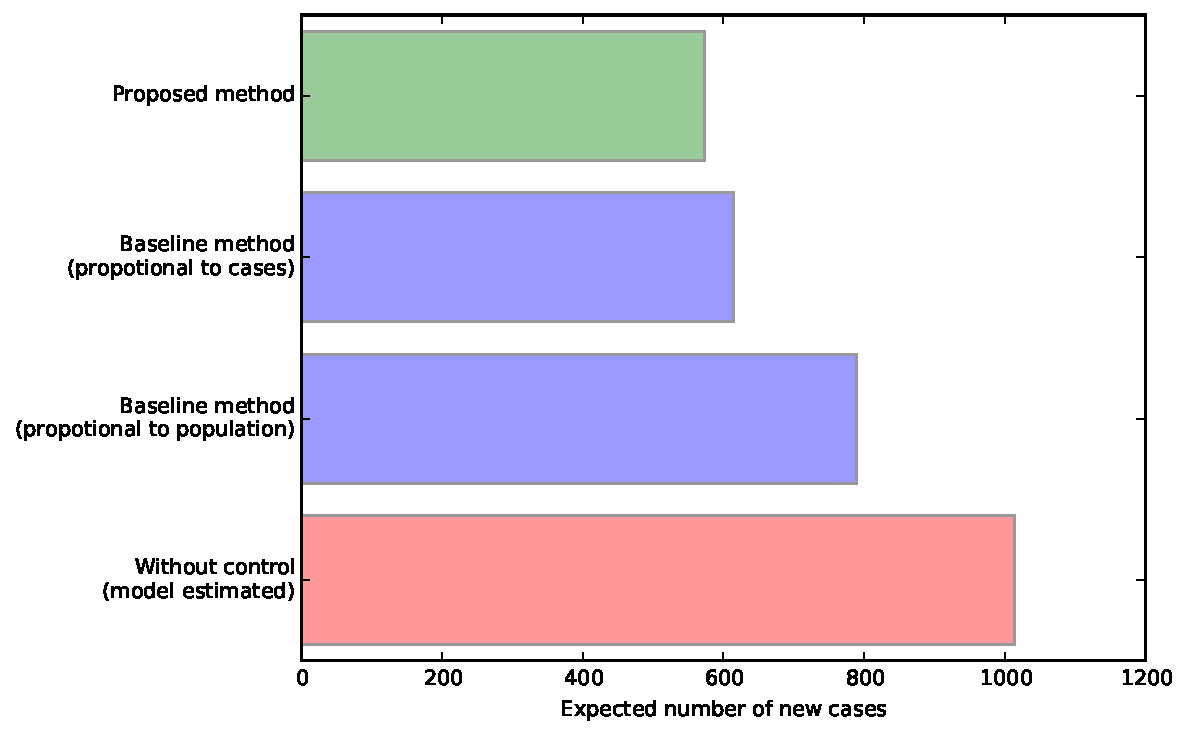
\includegraphics[width=4in]{graph/res2.pdf}
  \caption{Effect of different medication strategies}
  \label{med}
\end{center}  
\end{figure}


\begin{figure}[hbt]
\begin{center}
  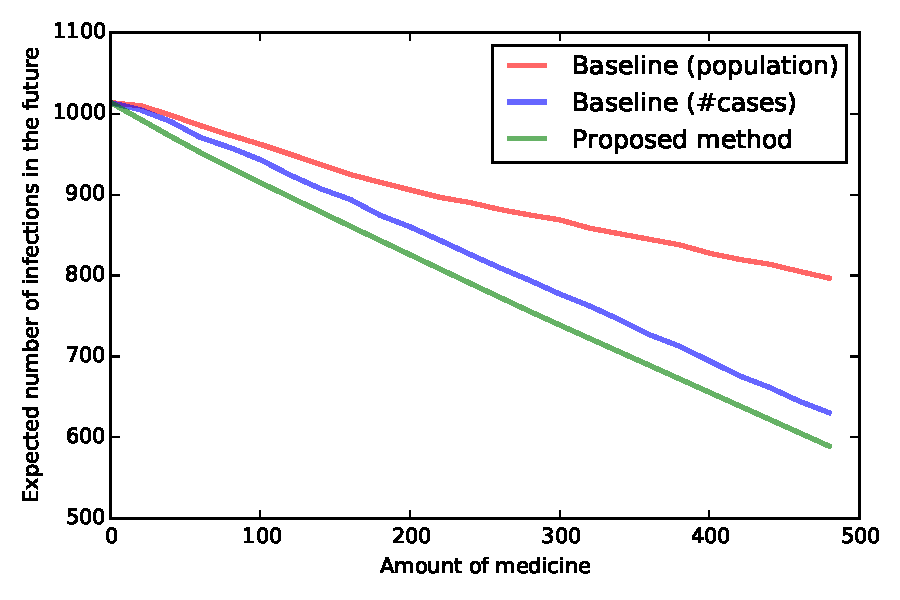
\includegraphics[width=4in]{graph/ev.pdf}
  \caption{Effect of different medication strategies over time}
  \label{ev}
\end{center}  
\end{figure}



\begin{figure}[hbt]
\begin{center}
  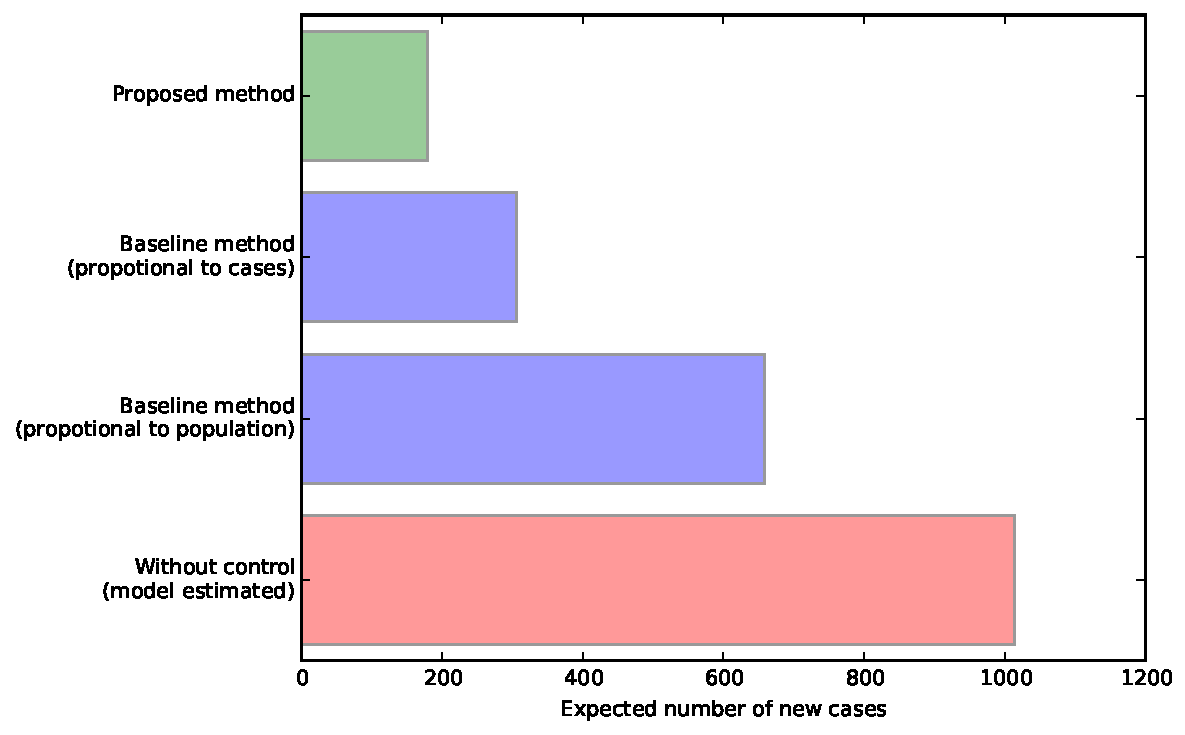
\includegraphics[width=4in]{graph/res4.pdf}
  \caption{Effect of different vaccination strategies}
  \label{med2}
\end{center}  
\end{figure}



\begin{figure}%[hbt]
\begin{center}
  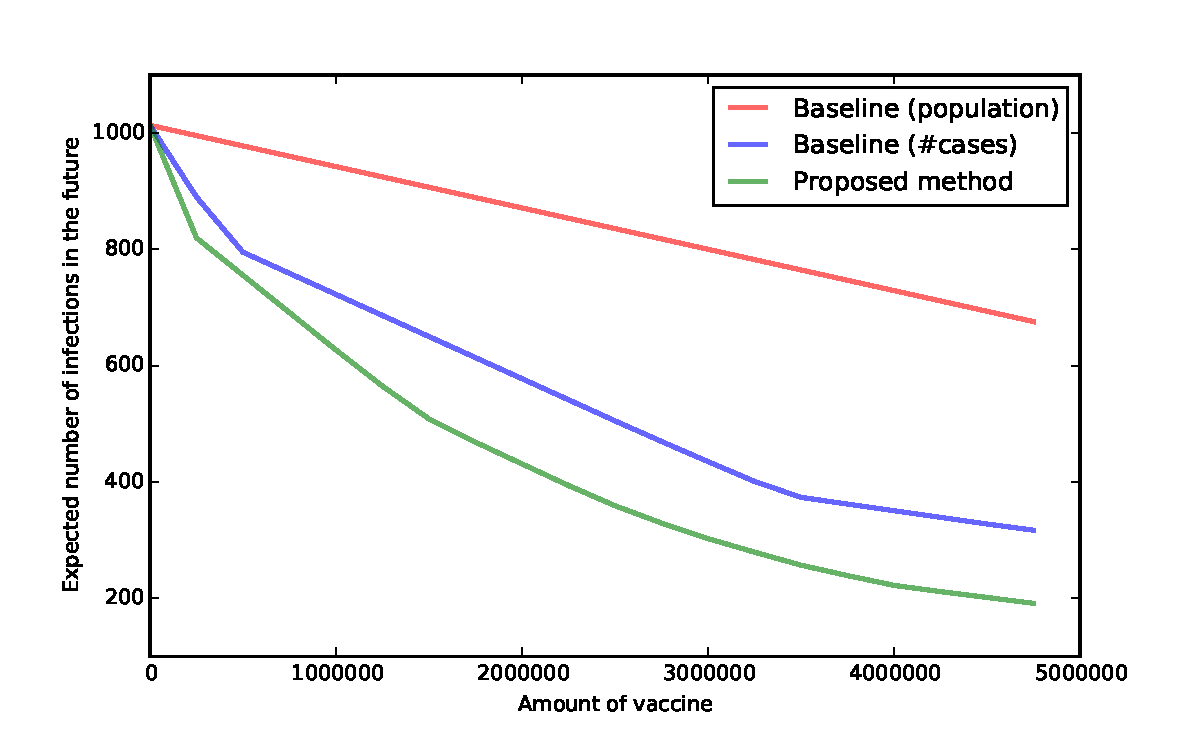
\includegraphics[width=4in]{graph/ev2.pdf}
  \caption{Effect of different vaccination strategies over time}
  \label{ev2}
\end{center}  
\end{figure}



\subsection{Disease Precautioning System}




\begin{figure}%[hbt]
\begin{center}
  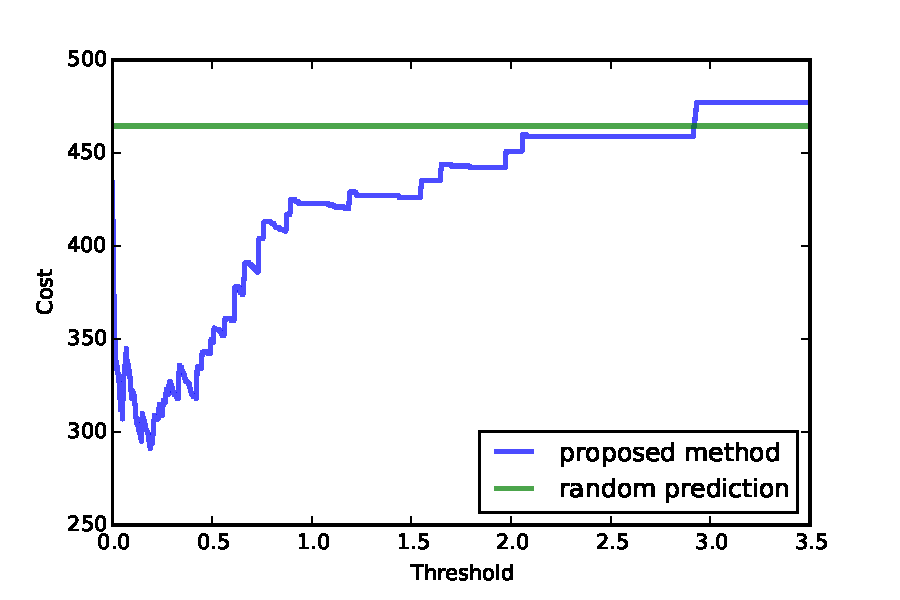
\includegraphics[width=4in]{graph/cost.pdf}
  \caption{Comparison to random prediction}
  \label{random}
\end{center}  
\end{figure}



\newpage
\bibliography{ref}
\bibliographystyle{ieeetr}


\newpage


\section*{Appendix}
\label{appendix}
Some large figures are plotted in this section.

\begin{figure}%[hbt]
\begin{center}
  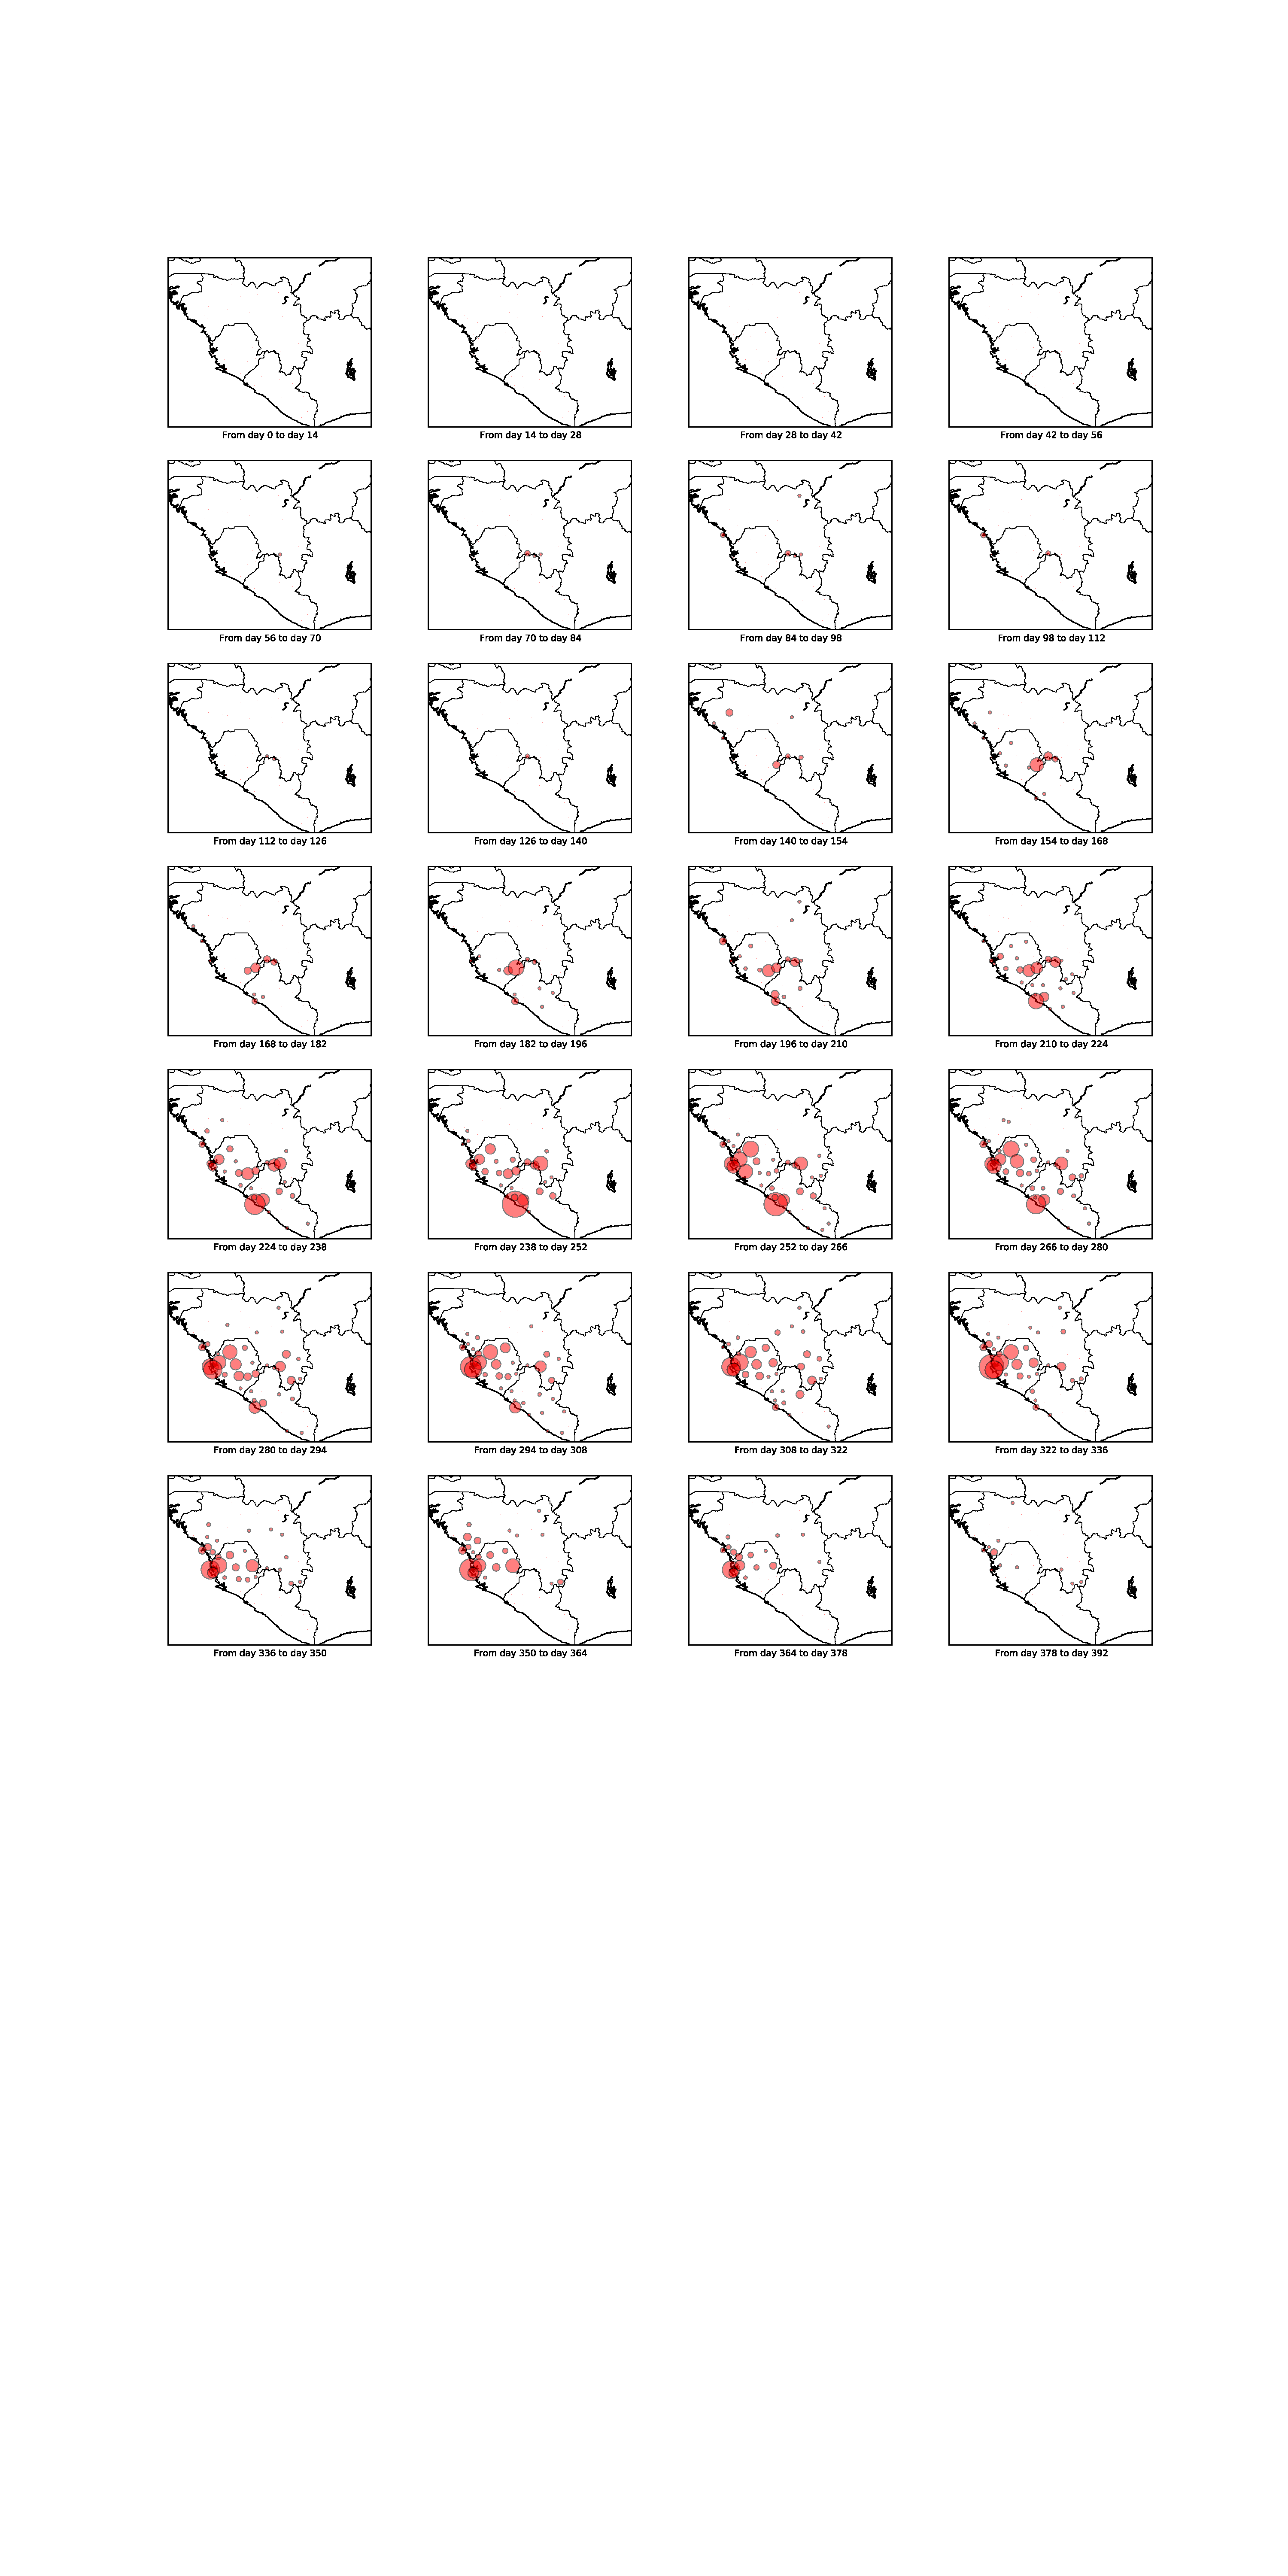
\includegraphics[width=6.1in]{graph/spread2.pdf}
  \caption{Spread of Ebola disease}
  \label{spread}
\end{center}  
\end{figure}




\end{document}